% Attention AE/ME. The following layout issues have not been checked by the English Editing Department and must be carefully verified by the AE/Layout Department: All callout issues, bold usage of callouts, and references to callouts in the text. Correct callout usage in figures. Figure and Table layout issues. Footnote formatting and Glossaries have not been checked. En dash usage for negative values, en dash usage to indicate relationships, en dash usage to indicate bonds (especially in chemistry). The English Editing Department is not responsible for correct italic usage for genes, proteins and technical terminology. This responsibility belongs to the authors. The following are also not checked: spacing between numbers and units of measurement, ratios, en dashes for ranges, date and time formats, punctuation in equation lines, and less than/more than spacing (< >). Finally, capitalization and layout of titles/headings must be properly checked as well as ensuring 'Eq.' and 'Fig.' are properly spelled out, as these are layout issues.

%  LaTeX support: latex@mdpi.com 
%  In case you need support, please attach all files that are necessary for compiling as well as the log file, and specify the details of your LaTeX setup (which operating system and LaTeX version / tools you are using).

%=================================================================
\documentclass[entropy,article,accept,moreauthors,pdftex]{Definitions/mdpi} 

\usepackage{amsthm}
\usepackage{amsmath}
\usepackage{amssymb}
\usepackage{bbm}
\usepackage{bookmark}
\usepackage{algorithmic}
\usepackage{algorithm}
\usepackage{graphicx}
\usepackage[labelformat=simple]{subcaption}
\renewcommand\thesubfigure{\alph{subfigure}}
\DeclareCaptionLabelFormat{subcaptionlabel}{\normalfont(\textbf{#2}\normalfont)}
\captionsetup[subfigure]{labelformat=subcaptionlabel}

%\newtheorem{theorem}{Theorem}
%\newtheorem{definition}{Definition}
%\newtheorem{corollary}{Corollary}
%\newtheorem{proposition}{Proposition}
%\newtheorem{lemma}{Lemma}
%\newtheorem{remark}{Remark}
\newcommand{\A}{\frac{a \log n}{n}}
\newcommand{\B}{\frac{b \log n}{n}}
\newcommand{\cG}{\mathcal{G}}
\newcommand{\cI}{\mathcal{I}}
\newcommand{\1}{\mathbbm{1}}
\DeclareMathOperator{\Var}{Var}
\DeclareMathOperator{\SSBM}{SSBM}
\DeclareMathOperator{\SIBM}{SIBM}
\DeclareMathOperator{\Dist}{dist}

% If you would like to post an early version of this manuscript as a preprint, you may use preprint as the journal and change 'submit' to 'accept'. The document class line would be, e.g., \documentclass[preprints,article,accept,moreauthors,pdftex]{mdpi}. This is especially recommended for submission to arXiv, where line numbers should be removed before posting. For preprints.org, the editorial staff will make this change immediately prior to posting.

%--------------------
% Class Options:
%--------------------
%----------
% journal
%----------
% Choose between the following MDPI journals:
% acoustics, actuators, addictions, admsci, adolescents, aerospace, agriculture, agriengineering, agronomy, ai, algorithms, allergies, analytica, animals, antibiotics, antibodies, antioxidants, applmech, applmicrobiol, applnano, applsci, arts, asc, asi, atmosphere, atoms, audiolres, automation, axioms, batteries, bdcc, behavsci, beverages, biochem, bioengineering, biologics, biology, biomechanics, biomedicines, biomedinformatics, biomimetics, biomolecules, biophysica, biosensors, biotech, birds, bloods, brainsci, breath, buildings, businesses, cancers, carbon, cardiogenetics, catalysts, cells, ceramics, challenges, chemengineering, chemistry, chemosensors, chemproc, children, civileng, cleantechnol, climate, clockssleep, cmd, coatings, colloids, compounds, computation, computers, condensedmatter, conservation, constrmater, cosmetics, crops, cryptography, crystals, cyber, dairy, data, dentistry, dermato, dermatopathology, designs, diabetology, diagnostics, digital, disabilities, diseases, diversity, dna, drones, dynamics, earth, ebj, ecologies, econometrics, economies, education, ejbc, ejihpe, electricity, electrochem, electronicmat, electronics, encyclopedia, endocrines, energies, eng, engproc, ent, entropy, environments, environsciproc, epidemiologia, epigenomes, est, fermentation, fibers, fire, fishes, fluids, foods, forecasting, forensicsci, forests, fractalfract, fuels, futureinternet, futureparasites, futurepharmacol, futurephys, galaxies, games, gases, gastroent, gastrointestdisord, gels, genealogy, genes, geographies, geohazards, geomatics, geosciences, geriatrics, hazardousmatters, healthcare, hearts, hemato, heritage, highthroughput, histories, horticulturae, humanities, hydrogen, hydrology, hygiene, idr, ijerph, ijfs, ijgi, ijms, ijns, ijtm, ijtpp, immuno, informatics, information, infrastructures, inorganics, insects, instruments, inventions, iot, j, jcdd, jcm, jcp, jcs, jdb, jfb, jfmk, jimaging, jintelligence, jlpea, jmmp, jmp, jmse, jne, jnt, jof, joitmc, jor, journalmedia, jox, jpm, jrfm, jsan, jtaer, jzbg, kidney, land, languages, laws, life, liquids, literature, livers, logistics, lubricants, machines, macromol, magnetism, magnetochemistry, make, marinedrugs, materials, materproc, mathematics, mca, measurements, medicina, medicines, medsci, membranes, metabolites, metals, micro, microarrays, micromachines, microorganisms, minerals, mining, modelling, molbank, molecules, mps, mti, nanomanufacturing, nanomaterials, ncrna, network, neuroglia, neurolint, neurosci, nitrogen, notspecified, nri, nursrep, nutrients, obesities, oceans, ohbm, oncopathology, optics, oral, organics, osteology, oxygen, parasites, particles, pathogens, pathophysiology, pediatric, pharmaceuticals, pharmaceutics, pharmacy, philosophies, photochem, photonics, physchem, physics, physiolsci, plants, plasma, pollutants, polymers, polysaccharides, preprints, proceedings, processes, prosthesis, proteomes, psych, psychiatryint, publications, quantumrep, quaternary, qubs, radiation, reactions, recycling, regeneration, religions, remotesensing, reports, reprodmed, resources, risks, robotics, safety, sci, scipharm, sensors, separations, sexes, sexes, signals, sinusitis, skins, smartcities, sna, societies, socsci, soilsystems, solids, sports, standards, stats, stresses, surfaces, surgeries, suschem, sustainability, symmetry, systems, taxonomy, technologies, telecom, test, textiles, thermo, tourismhosp, toxics, toxins, transplantology, transportation, traumas, tropicalmed, universe, urbansci, uro, vaccines, vehicles, vetsci, vibration, viruses, vision, water, wem, wevj, women, world

%---------
% article
%---------
% The default type of manuscript is "article", but can be replaced by: 
% abstract, addendum, article, benchmark, book, bookreview, briefreport, casereport, changes, comment, commentary, communication, conceptpaper, conferenceproceedings, correction, conferencereport, expressionofconcern, extendedabstract, meetingreport, creative, datadescriptor, discussion, editorial, essay, erratum, hypothesis, interestingimages, letter, meetingreport, newbookreceived, obituary, opinion, projectreport, reply, retraction, review, perspective, protocol, shortnote, supfile, technicalnote, viewpoint
% supfile = supplementary materials

%----------
% submit
%----------
% The class option "submit" will be changed to "accept" by the Editorial Office when the paper is accepted. This will only make changes to the frontpage (e.g., the logo of the journal will get visible), the headings, and the copyright information. Also, line numbering will be removed. Journal info and pagination for accepted papers will also be assigned by the Editorial Office.

%------------------
% moreauthors
%------------------
% If there is only one author the class option oneauthor should be used. Otherwise use the class option moreauthors.

%---------
% pdftex
%---------
% The option pdftex is for use with pdfLaTeX. If eps figures are used, remove the option pdftex and use LaTeX and dvi2pdf.

%=================================================================
\firstpage{1} 
\makeatletter 
\setcounter{page}{\@firstpage} 
\makeatother
\pubvolume{1}
\issuenum{1}
\articlenumber{0}
\pubyear{2021}
\copyrightyear{2020}
%\externaleditor{Academic Editor: Firstname Lastname}
\datereceived{29 November 2020} 
\dateaccepted{20 December 2020 } 
\datepublished{} 
\hreflink{https://doi.org/} % Please use \linebreak if need to do line break

%% MDPI internal command: uncomment if new journal that already uses continuous page numbers 
%\continuouspages{yes}

%------------------------------------------------------------------
% The following line should be uncommented if the LaTeX file is uploaded to arXiv.org
%\pdfoutput=1

%=================================================================
% Add packages and commands here. The following packages are loaded in our class file: fontenc, inputenc, calc, indentfirst, fancyhdr, graphicx,epstopdf, lastpage, ifthen, lineno, float, amsmath, setspace, enumitem, mathpazo, booktabs, titlesec, etoolbox, tabto, xcolor, soul, multirow, microtype, tikz, totcount, amsthm, hyphenat, natbib, hyperref, footmisc, url, geometry, newfloat, caption

%=================================================================
%% Please use the following mathematics environments: Theorem, Lemma, Corollary, Proposition, Characterization, Property, Problem, Example, ExamplesandDefinitions, Hypothesis, Remark, Definition, Notation, Assumption
%% For proofs, please use the proof environment (the amsthm package is loaded by the MDPI class).

%=================================================================
% Full title of the paper (Capitalized)
\Title{Exact Recovery of Stochastic Block Model by Ising Model}

\TitleCitation{Exact Recovery of Stochastic Block Model by Ising Model}

% Author Orchid ID: enter ID or remove command
%\newcommand{\orcidauthorA}{0000-0000-000-000X} % Add \orcidA{} behind the author's name
%\newcommand{\orcidauthorB}{0000-0000-000-000X} % Add \orcidB{} behind the author's name

% Authors, for the paper (add full first names)
\Author{{Feng Zhao} $^{1,\dagger}$, Min Ye $^{2,\dagger}$ and Shao-Lun~Huang {$^{2,}$}*}




% Authors, for metadata in PDF
\AuthorNames{Feng Zhao, Min Ye and Shao-Lun~Huang}

\AuthorCitation{Zhao, F.; Ye, M.;\linebreak Huang, S.-L.}

% Affiliations / Addresses (Add [1] after \address if there is only one affiliation.)
\address{%
$^{1}$ \quad Department of Electronics, Tsinghua University, Beijing 100084, China; zhaof17@mails.tsinghua.edu.cn\\
$^{2}$ \quad Tsinghua Berkeley Shenzhen Institute, Berkeley CA 94704, USA; yeemmi@sz.tsinghua.edu.cn}


% Contact information of the corresponding author
\corres{Correspondence: shaolun.huang@sz.tsinghua.edu.cn}

% Current address and/or shared authorship
\firstnote{These authors contributed equally to this work.} 
%\secondnote{}
% The commands \thirdnote{} till \eighthnote{} are available for further notes

%\simplesumm{} % Simple summary

%\conference{} % An extended version of a conference paper

% Abstract (Do not insert blank lines, i.e. \\) 
\abstract{In this paper, we study the phase transition property of an Ising model defined on a special random graph---the stochastic block model (SBM).
	Based on the Ising model, we propose a stochastic estimator to achieve the exact recovery for the SBM.
	The stochastic algorithm can be transformed into an optimization problem, which includes the special case of maximum likelihood
	and maximum modularity.
	Additionally, we give a consistent estimator for the model parameters of the SBM, which can be computed in constant time.
	Finally, we use metropolis sampling to realize the stochastic estimator and verify the phase transition phenomenon thfough experiments.}

% Keywords
\keyword{stochastic block model; exact recovery; Ising model; maximum likelihood; metropolis sampling}  % List three to ten pertinent keywords specific to the article, yet reasonably common within the subject discipline.

% The fields PACS, MSC, and JEL may be left empty or commented out if not applicable
%\PACS{J0101}
%\MSC{}
%\JEL{}

%%%%%%%%%%%%%%%%%%%%%%%%%%%%%%%%%%%%%%%%%%
% Only for the journal Diversity
%\LSID{\url{http://}}

%%%%%%%%%%%%%%%%%%%%%%%%%%%%%%%%%%%%%%%%%%
% Only for the journal Applied Sciences:
%\featuredapplication{Authors are encouraged to provide a concise description of the specific application or a potential application of the work. This section is not mandatory.}
%%%%%%%%%%%%%%%%%%%%%%%%%%%%%%%%%%%%%%%%%%

%%%%%%%%%%%%%%%%%%%%%%%%%%%%%%%%%%%%%%%%%%
% Only for the journal Data:
%\dataset{DOI number or link to the deposited data set in cases where the data set is published or set to be published separately. If the data set is submitted and will be published as a supplement to this paper in the journal Data, this field will be filled by the editors of the journal. In this case, please make sure to submit the data set as a supplement when entering your manuscript into our manuscript editorial system.}

%\datasetlicense{license under which the data set is made available (CC0, CC-BY, CC-BY-SA, CC-BY-NC, etc.)}

%%%%%%%%%%%%%%%%%%%%%%%%%%%%%%%%%%%%%%%%%%
% Only for the journal Toxins
%\keycontribution{The breakthroughs or highlights of the manuscript. Authors can write one or two sentences to describe the most important part of the paper.}

%%%%%%%%%%%%%%%%%%%%%%%%%%%%%%%%%%%%%%%%%%
% Only for the journal Encyclopedia
%\encyclopediadef{Instead of the abstract}

%\setcounter{secnumdepth}{4}
%%%%%%%%%%%%%%%%%%%%%%%%%%%%%%%%%%%%%%%%%%
\begin{document}
%%%%%%%%%%%%%%%%%%%%%%%%%%%%%%%%%%%%%%%%%%

%%%%%%%%%%%%%%%%%%%%%%%%%%%%%%%%%%%%%%%%%%
%\setcounter{section}{-1} %% Remove this when starting to work on the template.
%\section{How to Use this Template}
%The template details the sections that can be used in a manuscript. Note that the order and names of article sections may differ from the requirements of the journal (e.g., the positioning of the Materials and Methods section). Please check the instructions for authors page of the journal to verify the correct order and names. For any questions, please contact the editorial office of the journal or support@mdpi.com. For LaTeX related questions please contact latex@mdpi.com.
%The order of the section titles is: Introduction, Materials and Methods, Results, Discussion, Conclusions for these journals: aerospace,algorithms,antibodies,antioxidants,atmosphere,axioms,biomedicines,carbon,crystals,designs,diagnostics,environments,fermentation,fluids,forests,fractalfract,informatics,information,inventions,jfmk,jrfm,lubricants,neonatalscreening,neuroglia,particles,pharmaceutics,polymers,processes,technologies,viruses,vision

\section{Introduction}
In network analysis, community detection consists in inferring the group of vertices that
are more densely connected in a graph~\cite{fortunato2010community}. It has been used in many domains, such as recommendation systems~\cite{feng2015personalized},
task allocation in distributed computing~\cite{hendrickson2000graph}, gene expressions~\cite{cline2007integration}, and~so on.
The stochastic block model (SBM) is one of the most commonly used statistical models for community detection problems~\cite{holland1983stochastic, abbe2017community}.
It provides a benchmark artificial dataset to evaluate different community detection algorithms
and inspires the design of many algorithms for community detection tasks. These algorithms, such as
semi-definite relaxation, spectral clustering, and label propagation, not only have theoretical guarantees when applied to the SBM,
but also perform well on datasets without the SBM assumption. The~study of the theoretical guarantee of the SBM model can be divided between
the problem of exact recovery and that of partial recovery. Exact recovery requires that the estimated community should be exactly
the same as the underlining community structure of the SBM whereas partial recovery expects the ratio of misclassified nodes to be as small as possible.
For both cases, the~asymptotic behavior of the detection error
is analyzed when the scale of the graph tends to infinity. There are already some well-known results for the exact recovery problem
on the SBM.	To~name but a few, Abbe and Mossel established the exact recovery region for a special sparse SBM with two communities~\cite{abbe2015exact, mossel2016}.
Later on, the~result was extended to a general SBM with multiple communities~\cite{abbe2015community}.

Parameter inference in the  SBM is often considered alongside the exact recovery problem.
Previous inference methods require the joint estimation of node labels and model parameters~\cite{nowicki2001estimation}, which have high complexity since the recovery and inference tasks are done simultaneously.
In this article, we will decouple the inference and recovery problems, and propose a consistent estimator for SBM parameters when the number of communities is known. Once  the estimator is obtained, the~recovery condition can be checked to determine whether it is possible to recover the labels
exactly. Additionally, the~estimated parameter will guide the choice of parameters for our proposed stochastic~algorithm.

In this article, the~exact recovery of the SBM is analyzed by considering
the Ising model, which is a probability distribution of node states~\cite{ising1925beitrag}. We use the terms node states and node labels interchangeably throughout this paper, both of which refer to the membership of the underlining community. The
Ising model was originally proposed in statistical mechanics to model the ferromagnetism phenomenon but has wide applications in neuroscience, information theory,
and social networks. Among~different variants of Ising models, the~phase transition property is shared. Phase transition can be generally formulated when
some information quantity changes sharply in a small neighborhood of parameters.
Based on the random graph generated by an SBM with two underlining communities,
the connection of the SBM and the Ising model was first studied by~\cite{ye2020exact}. Our work will extend the existing result to the multiple community case, establish the phase transition
property, and give the recovery error an upper bound. The~error bounds decay in a polynomially fast rate in different phases.
Then we will propose an alternative approach to estimate the labels by finding the Ising state with maximal probability.
Compared with sampling from the Ising model directly,
we will show that the optimization approach has a sharper error upper bound. Solving the optimization problem
is a generalization of maximum likelihood and also has a connection with maximum modularity.
Additionally, searching the state with maximal probability
could also be done within all balanced partitions. We will show that this constrained search is equivalent to the  graph minimum cut problem, and~the detection
error upper bound for the constrained maximization will also be~given.

The exact solution to maximize the probability function or exact sampling from the Ising model is NP-hard. Many polynomial time algorithms have been proposed for approximation purposes.
Among these algorithms, simulated annealing performs well and produces a solution that is very close to the true maximal value~\cite{liu2010detecting}.
On the other hand, in~the original Ising model,
metropolis sequential sampling is used to generate samples for the  Ising model~\cite{metropolis1953equation}. Simulated annealing can be regarded as metropolis sampling with decreasing temperature. In~this article, we will
use the metropolis sampling technique to sample from the Ising model defined on the SBM. %confirm.
This approximation enables us to verify the phase transition property of our Ising model~numerically.

This paper is organized as follows. Firstly, in~Section~\ref{sec:psbm} we introduce the SBM and give an estimator for the parameters of the SBM.
Then, in  Section~\ref{sec:sibm}, our specific Ising model is given and its phase transition property is obtained.
Derived from the Ising model,\linebreak in~Section~\ref{sec:em}, the~energy minimization method is introduced, and~we establish its connection with maximum likelihood and modularity
maximization algorithm. Furthermore, in~Section~\ref{sec:ms},
we realize the Ising model using the metropolis algorithm to generate samples. Numerical experiments and conclusion are given lastly to finish this~paper.

Throughout this paper, the~  community number is denoted by $k$;
the random undirected graph $G$ is written as $G(V,E)$ with vertex set $V$ and edge set $E$;
$V=\{1,\dots, n\} =: [n]$;
the label of each node is $X_i$, which is chosen from $W= \{1, \omega, \dots, \omega^{k-1}\}$, and we further require $W$
to be a cyclic group with order $k$;
$W^n$ is the n-ary Cartesian power of $W$; % see https://en.wikipedia.org/wiki/Cartesian_product#n-ary_Cartesian_power
$f$ is a permutation function on $W$ and is extended to $W^n$ in an element-wise manner;
$U^c$ is the complement set of $U$ and $|U|$ is the cardinality of $U$;  
the set $S_k$ is used to represent all permutation functions on $W$ and $S_k(\sigma):=\{f(\sigma)| f\in S_k\}$ for $\sigma \in W^n$;
the indicator function $\delta(x,y)$ is defined as
$\delta(x,y) = 1 $ when $x=y$, and~$\delta(x,y)=0$ when $x\neq y$;
$f(n) = O(g(n))$ if there exists a constant $c > 0$ such that $ f(n) \leq c g(n)$
for large $n$; $f(n)=o(g(n))$ holds if $\lim_{n\to\infty} \frac{f(n)}{g(n)} = 0$;
we define the distance of two vectors as:
$\Dist(\sigma, \sigma')
=|\{i\in[n]:\sigma_i\neq \sigma'_i\}| \textrm{ for } \sigma,\sigma'\in W^n
$ and the distance of a vector to a space $S\subseteq W^n$
as
$\Dist(\sigma,S)
:=\min\{\Dist(\sigma, \sigma') | \sigma' \in S\}
$. For~example, when $n=2$ and $k=2$, $\sigma=(1, \omega) \in W^2$;
$\omega^0 = 1$; $\omega \cdot \omega = \omega^2 = 1$; let $f$ be a mapping such that $f(1) = \omega$ and $f(\omega)=1$,
then $f \in S_2$ and $f(\sigma) = (\omega, 1)$; $\Dist(\sigma, f(\sigma)) = 2$; $S_k(\sigma) = \{\sigma, f(\sigma)\}$; and
$S_k^c(\sigma) = \{(1, 1), (\omega, \omega)\}$.
%%%%%%%%%%%%%%%%%%%%%%%%%%%%%%%%%%%%%%%%%%
\section{Related~Works}
The classical Ising model is defined on a lattice and confined to two states $\{\pm 1\}$. This definition
can be extended to a general graph and multiple-state case~\cite{potts1952some}. In~\cite{liu2017log}, Liu considered
the Ising model as defined on a graph generated by sparse SBM and his focus was to compute the log partition function,
which was averaged over all random graphs. In~\cite{berthet2019exact}, an~Ising model with a repelling interaction
was considered on a fixed graph structure, and~the phase transition condition was established, which involves both the attracting and repelling
parameters. Our Ising model derives from the work of~\cite{ye2020exact}, but~we extend their results by considering the error upper bound and
multiple-community~case.

The exact recovery condition for the SBM can be derived as a special case of many generalized models, such as pairwise measurements~\cite{chen2016information},
minimax rates~\cite{hajek2016achieving}, and side information~\cite{saad2018community}. The Ising model in this paper provides another way to extend the
SBM model and derives the recovery condition. Additionally,
the error upper bound for exact recovery of\linebreak the two-community SBM by constrained maximum likelihood has been obtained in~\cite{abbe2015exact}.
Compared with previous results, we establish a sharper upper bound for the multiple-community case in this~paper.

The connection between maximum modularity and maximal likelihood was investigated in~\cite{newman2016equivalence}. To~get an optimal value
of maximum modularity approximately, simulated annealing was exploited~\cite{he2016fast}, which proceeds by using the partition approach, while the Metropolis sampling
used in this paper is applied to estimate the node membership~directly.

%%%%%%%%%%%%%%%%%%%%%%%%%%%%%%%%%%%%%%%%%%
\section{Stochastic Block Model and Parameter~Estimation}\label{sec:psbm}
In this paper, we consider a special symmetric stochastic block model (SSBM), which is defined as follows:
	\begin{Definition}[SSBM with $k$ communities] \label{def:SSBM}
	Let $0\leq q<p\leq 1$, $V=[n]$ and\linebreak $X=(X_1,\dots,X_n)\in W^n$. $X$ satisfies the constraint that $|\{v \in [n] : X_v = u\}| = \frac{n}{k}$ for $u\in W$.
	The random graph $G$ is generated under $\SSBM(n,k,p,q)$ if the following two conditions are~satisfied.
	\begin{enumerate}
	\item There is an edge of $G$ between the vertices $i$ and $j$ with probability $p$ if $X_i=X_j$ and with probability $q$ if $X_i \neq X_j$.
	\item The existences of each edge are mutually independent.
	\end{enumerate}
\end{Definition}
To explain SSBM in more detail,
we define the random variable $Z_{ij}:=\mathbbm{1}[\{i,j\} \in E(G)]$, which is the indicator function of the existence of an edge between nodes $i$ and $j$.
Given the node labels $X$, $Z_{ij}$ follows Bernoulli distribution, whose expectation is given by:
\begin{equation}
\mathbb{E}[Z_{ij}] =
\begin{cases}
p & \textrm{ if } X_i = X_j \\ 
q & \textrm{ if }  X_i \neq X_j
\end{cases}
\end{equation}

Then the random graph $G$ with $n$ nodes
is completely specified by\linebreak $Z:=\{Z_{ij}, 1\leq i<j\leq n\}$ in which all $Z_{ij}$ are jointly independent.
The probability distribution for SSBM can be written as:
\begin{align}
&P_G(G):=P_G(Z = z| X) = p^{\sum_{X_i = X_j} z_{ij}}q^{\sum_{X_i \neq X_j} z_{ij}} \notag \\
&\quad \cdot (1-p)^{\sum_{X_i = X_j} (1-z_{ij})}(1-q)^{\sum_{X_i \neq X_j} (1-z_{ij})} \label{eq:GmL}
\end{align}

We will use the notation $\cG_n$ to represent the set containing all graphs with $n$ nodes. By~the normalization property,
$P_G(\cG_n) = \sum_{G\in \cG_n}P_G(G)=1$.

In Definition \ref{def:SSBM}, we have supposed that the node label $X$ is fixed instead of a uniformly distributed random variable.
Since the maximum posterior estimator is equivalent to the maximum likelihood when the prior is uniform,
these two definitions are equivalent. Although~the random variable definition is more commonly used in previous literature~\cite{abbe2017community}, fixing $X$ makes our formal analysis more~concise.

Given the SBM, the~exact recovery problem can be formally defined as follows:
\begin{Definition}[Exact recovery in SBM] \label{def:SSBMR}
Given $X$, the~random graph $G$ is drawn under\linebreak $\SSBM(n,k,p,q)$. We say that the exact recovery is solvable for $\SSBM(n,k,p,q)$ if there exists an algorithm that takes
$G$ as input and outputs $\hat{X}$ such that:
\begin{equation*}
P_a(\hat{X}):=P(\hat{X} \in S_k(X)) \to 1 \textrm{ as } n \to \infty
\end{equation*}
\end{Definition}

In the above definition, the~notation $P_a(\hat{X})$ is called the probability of accuracy for estimator $\hat{X}$.
Let $P_e(\hat{X}) = 1 - P_a(\hat{X})$ represent the probability of error. Definition \ref{def:SSBMR} can also
be formulated as $P_e(\hat{X}) \to 0$ as $n\to \infty$.
The notation $\hat{X} \in S_k(X)$ means that we can only
expect a recovery up to a global permutation of the ground truth label vector $X$. This is common in unsupervised
learning as no anchor exists to assign labels to different communities.
Additionally, given a graph $G$, the~algorithm can
be either deterministic or stochastic. Generally speaking, the~probability of $\hat{X} \in S_k(X)$ should be understood as 
$\sum_{G \in \cG_n} P_G(G) P_{\hat{X}|G}(\hat{X} \in S_k(X))$, which reduced to 
$P_G(\hat{X} \in S_k(X))$ for the deterministic~algorithm.

For constants $p,q$, which are irrelevant with the graph size $n$,
we can always find algorithms to recover $X$ such that the detection error decreases exponentially
fast as $n$ increases; that is to say, the~task with a dense graph is relatively easy to handle. Within~this paper, we consider a sparse
case when $p = \A, q = \B$. This case corresponds to the sparsest graph when exact recovery of the SBM is possible.
And under this condition, a~well known result~\cite{abbe2015community} states that
exact recovery is possible if and only if:
\begin{equation}\label{eq:abk}
\sqrt{a} - \sqrt{b} > \sqrt{k}
\end{equation}

In the following, we assume \eqref{eq:abk} always hold,
and before diving into the exact recovery problem, we first consider the inference problem for SBM.
Suppose $k$ is known, and~we want to estimate $a,b$ from the graph $G$.
We offer a simple method
by counting the number of edges $T_1$ and the number of triangles $T_2$ of $G$, and~the estimators $\hat{a}, \hat{b}$ are
obtained by solving the following equation systems:
\begin{align}
\frac{x+(k-1)y}{2k} & = \frac{T_1}{n\log n} \label{eq:e_1}\\
\frac{1}{k^2}
\left(\frac{x^3}{6} + \frac{k-1}{2}xy^2 + (k-1)(k-2)\frac{y^3}{6}\right) & = \frac{T_2}{\log^3 n} \label{eq:e_2}
\end{align}

The theoretical guarantee for the solution is given by the following theorem:
\begin{Theorem}\label{thm:ab12}
When $n$ is large enough, the~equation system of Equations (\ref{eq:e_1}) and (\ref{eq:e_2}) has the  unique solution $(\hat{a}, \hat{b})$,
which are consistent estimators
of $(a,b)$. That is $\hat{a}, \hat{b}$ converge to $a,b$ in probability, respectively.
\end{Theorem}
Given a graph generated by the SBM, we can use Theorem \ref{thm:ab12} to obtain the estimated $a,b$ and determine whether
exact recovery of label $X$ is possible by Equation \eqref{eq:abk}. Additionally,  Theorem \ref{thm:ab12} provides good estimation of $a,b$ to initialize their parameters of
some recovery algorithm like maximum likelihood or our proposed Metropolis sampling in Section~\ref{sec:ms}.


\section{Ising Model for Community~Detection}\label{sec:sibm}
In the previous section, we have defined SBM and its exact recovery problem.  While SBM is regarded as obtaining
the graph observation $G$ from node label $X$, the Ising model provides a way to generate estimators of $X$ from $G$
by a stochastic procedure. The~definition of such an Ising model is given
as follows:
\begin{Definition}[Ising model with $k$ states]\label{def:ising}
	Given a graph $G$ sampled from\linebreak $\SSBM(n,k,\A,\B)$, the~Ising model with parameters $\gamma,\beta>0$
	is a probability distribution of the state vector $\sigma\in W^n$ whose probability mass function is
\begin{align} \label{eq:isingma}
	P_{\sigma|G}(\sigma=\bar{\sigma})=\frac{\exp(-\beta H(\bar{\sigma}))}{Z_G(\gamma,\beta)}
	\end{align}
	where
\begin{equation}\label{eq:energy}
	H(\bar{\sigma}) = \gamma \frac{\log n}{n} \sum_{\{i,j\}\not\in E(G)} \delta(\bar{\sigma}_i, \bar{\sigma}_j)
	- \sum_{\{i,j\}\in E(G)} \delta(\bar{\sigma}_i, \bar{\sigma}_j)
	\end{equation}
	
	The subscript in $P_{\sigma|G}$ indicates that the distribution depends on $G$, and~	$Z_G(\gamma,\beta)$ is the normalizing constant for this distribution.
\end{Definition}
In physics, $\beta$ refers to the inverse temperature and $Z_G(\gamma, \beta)$ is called the partition function.
The Hamiltonian energy $H(\bar{\sigma})$ consists of two terms: the repelling interaction between nodes without edge connection
and the attracting interaction between nodes with edge connection. The~parameter $\gamma$ indicates the ratio of the strength of these two
interactions. The~term $\frac{\log n}{n}$ is added to balance the two interactions because there are only $O(\frac{\log n}{n})$
connecting edges for each node.
The probability of each state is proportional to $\exp(-\beta H(\bar{\sigma}))$, and~the state with the largest
probability corresponds to that with the lowest~energy.

The classical definition of the Ising model is specified by $H(\sigma)=-\sum_{(i,j)\in E(G)} \sigma_i \cdot \sigma_j$ for
$\sigma_i = \pm 1$.
There are two main differences between Definition \ref{def:ising} and the classical one. Firstly, we add a repelling term
between nodes without an edge connection. This makes these nodes have a larger probability to take different labels.
Secondly, we allow the state at each node to take $k$ values from $W$ instead of the two values $\pm 1$.
When $\gamma = 0$ and $k=2$,\linebreak Definition \ref{def:ising}
is reduced to the classical definition of the Ising model up to a scaling~factor.

Definition \ref{def:ising} gives a stochastic estimator $\hat{X}^*$ for $X$: $\hat{X}^*$ is one sample generated from the Ising model, which is denoted as
$\hat{X}^* \sim \textrm{Ising}(\gamma, \beta)$.
The exact recovery error probability for $\hat{X}^*$ can be written as $P_e(\hat{X}^*) := \sum_{G \in \cG_n} P_G(G) P_{\sigma | G}(S^c_k(X))$. From~this expression we can see that the error probability is determined
by two parameters $(\gamma, \beta)$. When these parameters take proper values, $ P_e(\hat{X}^*)\to 0$, and the exact recovery of the SBM is achievable. On~the contrary, $P_e(\hat{X}^*) \to 1$ if $(\gamma, \beta)$ takes other values.
These two cases are summarized in the following theorem:
\begin{Theorem}\label{thm:phase_transition}
Define the function $g(\beta), \tilde{g}(\beta)$ as follows:
\begin{equation}
g(\beta) = \frac{be^{\beta} + a e^{-\beta}}{k} - \frac{a+b}{k} +1
\end{equation}
and:
\begin{equation}
\tilde{g}(\beta) = \begin{cases}
g(\beta) & \beta \leq \bar{\beta} = \frac{1}{2}\log \frac{a}{b} \\
g(\bar{\beta}) = 1 - \frac{(\sqrt{a} - \sqrt{b})^2}{k} & \beta > \bar{\beta}
\end{cases}
\end{equation}
where $\bar{\beta} =  \arg\min_{\beta > 0} g(\beta)$.
Let $\beta^*$ be defined as:
\begin{equation}\label{eq:beta_star}
\beta^* = \log\left(\frac{a + b - k - \sqrt{(a + b - k)^2 - 4 a b)}}{2  b}\right)
\end{equation}
which is the solution to the equation $g(\beta) = 0$ and $\beta^* < \bar{\beta}$. Then depending on
how $(\gamma, \beta)$ take values, for~any given $\epsilon > 0$ and $\hat{X}^* \sim \textrm{Ising}(\gamma, \beta)$, when $n$ is sufficiently large, we~have:
\begin{enumerate}
\item If $\gamma > b$ and $\beta > \beta^*$,  $P_e(\hat{X}^*) \leq n^{\tilde{g}(\beta)/2 + \epsilon}$;
\item If $\gamma > b$ and $\beta < \beta^*$, $P_a(\hat{X}^*) \leq (1+o(1))\max\{n^{g(\bar{\beta})}, n^{-g(\beta) + \epsilon}\}$;
\item If $\gamma < b$, $P_a(\hat{X}^*) \leq \exp(-C n)$ for any $C>0$.
\end{enumerate}
\end{Theorem}
By simple calculus, $\tilde{g}(\beta) < 0$ for $\beta> \beta^*$ and $g(\beta)>0$ for $\beta < \beta^*$. $g(\bar{\beta}) < 0$ follows from Equation \eqref{eq:abk}. The~illustration of $g(\beta), \tilde{g}(\beta)$ is shown in Figure~\ref{fig1}a.
Therefore, for~sufficiently small $\epsilon$ and as $n \to \infty$, the~upper bounds in Theorem \ref{thm:phase_transition} all converge to $0$ at least
in polynomial speed.
In this way, Theorem \ref{thm:phase_transition} establishes the sharp phase transition property of the Ising model, which is illustrated
in Figure~\ref{fig1}b.
% start a new page without indent 4.6cm
%\clearpage
\end{paracol}
\nointerlineskip
\begin{figure}[H]
\widefigure
\begin{subfigure}{0.43\textwidth}
	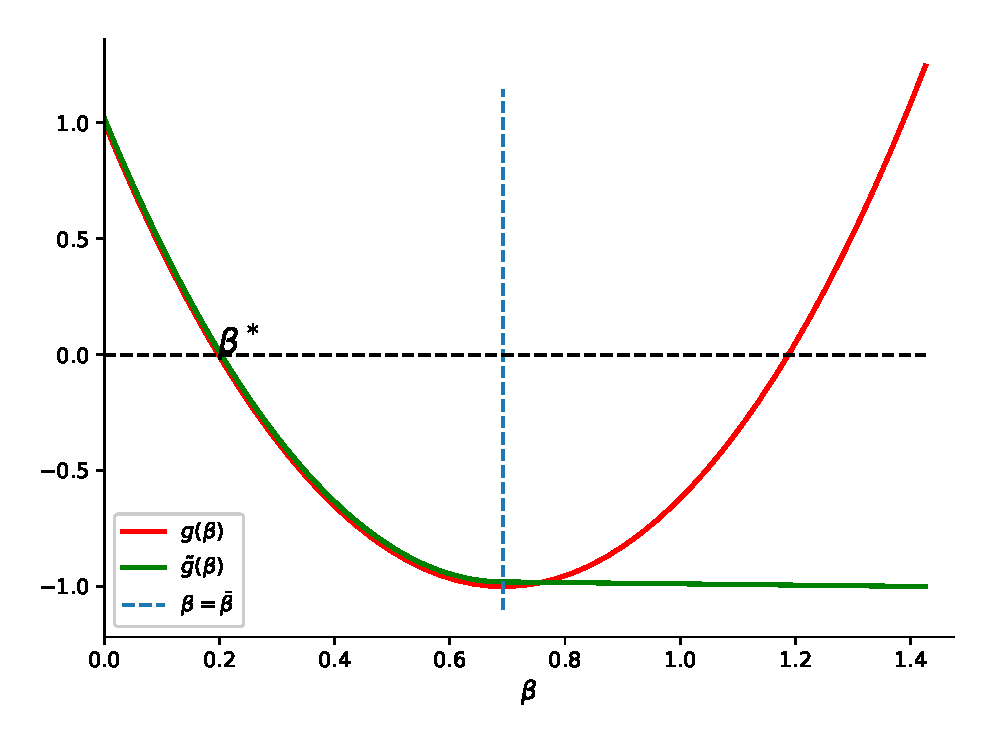
\includegraphics[width=\textwidth]{g-16-4-2.eps}
	\caption{$g(\beta),\tilde{g}(\beta)$ when $a=16,b=4,k=2$.}\label{fig:g}
\end{subfigure} 
\begin{subfigure}{0.5\textwidth}
	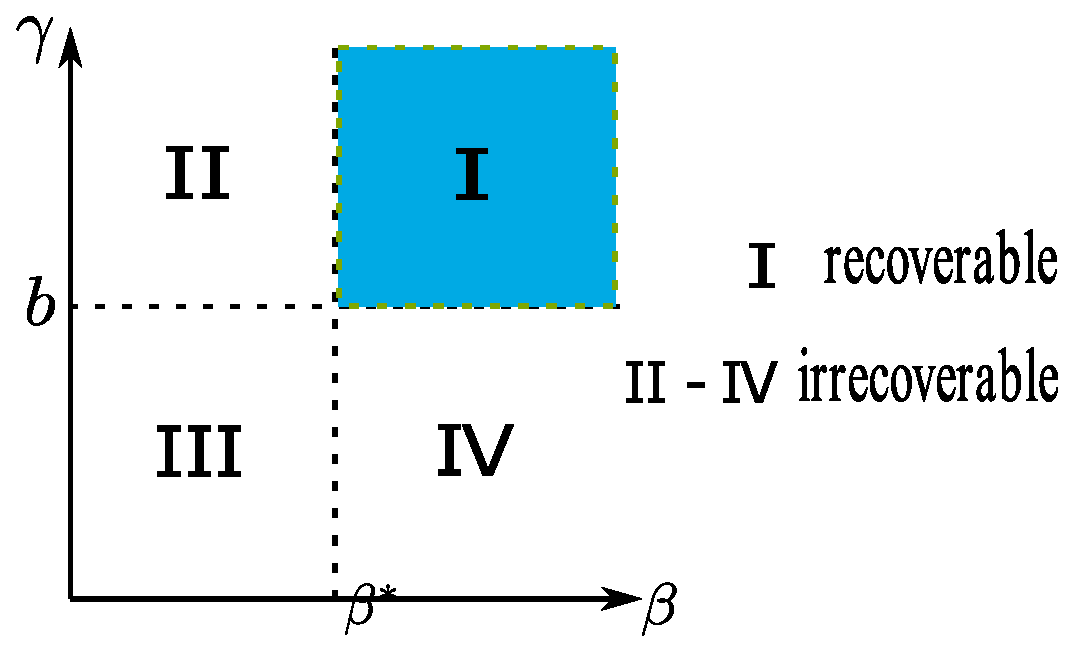
\includegraphics[width=\textwidth]{phase_trans.eps}
	\caption{Phase transition region in $(\beta, \gamma)$ plane.
	The exact recovery of the SSBM %please define.
	is solvable only in Region I.}\label{fig:pt}
\end{subfigure}
\caption{Illustration of Theorem \ref{thm:phase_transition}.}\label{fig1}
\end{figure}
\begin{paracol}{2}
%\linenumbers
\switchcolumn


Theorem
\ref{thm:phase_transition} can also be understood from the marginal distribution for\linebreak $\sigma: P_{\sigma}(\sigma =\bar{\sigma})
=\sum_{G \in \cG_n}P_G(G)P_{\sigma |G}(\sigma=\bar{\sigma})$.
Let $D(\sigma, \sigma')$ be the event when $\sigma$ is closest to $\sigma'$ among all its permutations.
That is,
\begin{equation}
D(\sigma, \sigma') := \{ \sigma = \arg\min_{f \in S_k} \Dist(f(\sigma), \sigma')  \}
\end{equation}

Then Theorem \ref{thm:phase_transition} can be stated with respect to the marginal distribution $P_{\sigma}$:
\begin{Corollary}\label{cor:phase4}
Suppose $\gamma > b$, depending on how $\beta$ takes~values:
\begin{enumerate}
	\item When $\beta > \beta^*$, $P_{\sigma}(\sigma = X | D(\sigma, X))  = 1-o(1)$;
	\item When $\beta < \beta^*$, $P_{\sigma}(\sigma = X | D(\sigma, X))  = o(1)$.
\end{enumerate}
\end{Corollary}

Below we outline the proof ideas of Theorem \ref{thm:phase_transition}. The~insight is obtained from the analysis of the one-flip energy difference.
This useful result is summarized in the following~lemma:
\begin{Lemma}\label{lem:lemmaDiff}
	Suppose $\bar{\sigma}'$ differs from $\bar{\sigma}$ only at position $r$ by $\bar{\sigma}'_r = \omega^s \cdot \bar{\sigma}_r$.
	Then the change of energy~is:
\begin{align}
	H(\bar{\sigma}') - H(\bar{\sigma}) &= (1+\gamma \frac{\log n}{n})\sum_{i \in N_r(G)} J_s(\bar{\sigma}_r, \bar{\sigma}_i)
	\notag \\
	&+ \gamma \frac{\log n}{n} (m(\omega^s \cdot \bar{\sigma}_r)-m(\bar{\sigma}_r)+1) \label{eq:DeltaH}
	\end{align}
	where $m(\omega^j) := |\{i \in [n] | \bar{\sigma}_i = \omega^j | \}$, $N_r(G):=\{j | (r, j) \in E(G) \}$ and $J_s(x, y) = \delta(x, y) - \delta(\omega_s \cdot x, y)$.
\end{Lemma}
Lemma \ref{lem:lemmaDiff} gives an explicit way to compare the probability of two neighboring states by the following
equality:
\begin{equation}\label{eq:Pratio}
\frac{P_{\sigma |G } (\sigma = \bar{\sigma}')}{P_{\sigma |G } (\sigma = \bar{\sigma})}
= \exp(-\beta(H(\bar{\sigma}') - H(\bar{\sigma})))
\end{equation}

Additionally, since the graph is sparse and every node has $O(\log n)$ neighbors, from Equation~\eqref{eq:DeltaH} the computational cost (time complexity) for the energy difference
is also $O(\log n)$. 

When $H(\bar{\sigma}') > H(\bar{\sigma})$, we can expect $P_{\sigma | G}(\sigma = \bar{\sigma}')$ is far less than 
$P_{\sigma | G}(\sigma = \bar{\sigma})$.
Roughly speaking, if~ $ \sum_{\Dist(\sigma', X)=1}\exp(-\beta(H(\bar{\sigma}') - H(X))) $ converges to zero,
we can expect the probability of all other states differing from $S_k(X)$ converges to zero.
On the contrary, if~$ \sum_{\Dist(\sigma', X)=1}\exp(-\beta(H(\bar{\sigma}') - H(X))) $ tends to infinity,
then  $P_{\sigma}(S_k(X))$ converges to zero. This illustrates the idea behind
the proof of
Theorem \ref{thm:phase_transition}. The~rigorous proof can be found in Section~\ref{sec:pm}.


\section{Community Detection via Energy~Minimization}\label{sec:em}
Since $\beta^*$ is irrelevant with $n$, when $\gamma>b$, we can choose a sufficiently large $\beta$ such that
$\beta > \beta^*$, then by Theorem \ref{thm:phase_transition}, $\sigma \in S_k(X)$ almost surely, which
implies that $P_{\sigma | G}(\sigma = X)$ has the largest value for almost all graphs $G$ sampled from the SBM. Therefore, instead of
sampling from the Ising model, we can directly maximize the conditional probability to find the state with the largest probability.
Equivalently, we can proceed by minimizing the energy term in Equation \eqref{eq:energy}:
\begin{equation}\label{eq:hatX}
\hat{X}' := \arg\min_{\bar{\sigma} \in W^n} H(\bar{\sigma})
\end{equation}

In \eqref{eq:hatX}, we allow $\bar{\sigma}$ to take values from $W^n$. Since we know $X$ has equal
size\linebreak $|\{v \in [n] : X_v = u\}| = \frac{n}{k}$ for each label $u$, another formulation is to restrict the search space to
$W^*:= \{\sigma\in W^n \big\vert |\{v \in [n] : \sigma_v = \omega^s\}| = \frac{n}{k}, s=0,\dots, k-1 \}$.
When $\sigma \in W^*$, minimizing $H(\sigma)$ is equivalent to:
\begin{equation}
\hat{X}'' := \arg\min_{\sigma \in W^*} \sum_{\{i,j\} \not\in E(G) } \delta(\sigma_i, \sigma_j)
\end{equation}
where the minimal value is the minimum cut between different detected~communities.

When $\hat{X}'' \neq X$, we must have $\Dist(\hat{X}'' ,X)\geq 2$ to satisfy the constraint $\hat{X}'' \in W^*$.
Additionally, the~estimator of $\hat{X}''$ is parameter-free whereas $\hat{X}'$ depends on $\gamma$. The~extra parameter $\gamma$ in the expression of
$\hat{X}'$ can be regarded as a kind of Lagrange multiplier for this integer programming problem. Thus, the~optimization problem for $\hat{X}'$
is the relaxation of that for $\hat{X}''$ by introducing a penalized term and enlarging the searched space from $W^*$ to $W^n$.

When $\beta > \bar{\beta}$, $\tilde{g}(\beta)$ becomes a constant value. Therefore, we can get $n^{g(\bar{\beta})/2}$ as the tightest error upper bound for the Ising estimator $\hat{X}^*$ from Theorem \ref{thm:phase_transition}.
For the estimator $\hat{X}'$ and $\hat{X}''$, we can obtain a sharper error upper bound, which is
summarized in the following theorem:
\begin{Theorem}\label{thm:error_rate}
When $\sqrt{a} - \sqrt{b} > \sqrt{k}$, for sufficiently~large~$n$, 
\begin{enumerate}
	\item If $\gamma > b$, $P_G(\hat{X}' \not\in S_k(X)) \leq (k-1+o(1))n^{g(\bar{\beta})}$;
	\item $P_G(\hat{X}'' \not\in S_k(X)) \leq ((k-1)^2+o(1))n^{2g(\bar{\beta})}$.
\end{enumerate}
\end{Theorem}
As $g(\bar{\beta})<0$, $n^{2g(\bar{\beta})} < n^{g(\bar{\beta})} < n^{g(\bar{\beta})/2}$,
Theorem \ref{thm:error_rate} implies that $P_e(\hat{X}'')$ has the sharpest upper bound among the three estimators.
This can be intuitively understood as the result of smaller search space.
The proof technique of Theorem \ref{thm:error_rate} is to consider the probability of events $H(X) > H(\bar{\sigma})$
for $\Dist(\bar{\sigma}, X) \geq 1$. Then by union bound, these error probabilities can be summed up.
We note that a loose bound $n^{g(\bar{\beta})/4}$ was obtained in~\cite{abbe2015exact} for the estimator $\hat{X}''$ when $k=2$.
For a general case, since $\tilde{g}(\beta) = 1- \frac{(\sqrt{a} - \sqrt{b})^2}{k}$, Theorem \ref{thm:error_rate} implies that exact recovery is possible using $\hat{X}'$ as long as  
$\sqrt{a} - \sqrt{b} > \sqrt{k}$ is~satisfied.


Estimator $\hat{X}'$ has one parameter, $\gamma$. When $\gamma$ takes different values, $\hat{X}'$
is equivalent with maximum likelihood or maximum modularity in the asymptotic case. The~following analysis shows
their relationship~intuitively.

The maximum likelihood estimator is obtained by maximizing the log-likelihood function.
From \eqref{eq:GmL}, this function can be written as:
$$
\log P_G(Z|X=\sigma) = -\log\frac{a}{b} \cdot H(\sigma) + C
$$
where the parameter $\gamma$ in $H(\sigma)$ satisfies \mbox{$\gamma \frac{\log n}{n} = \frac{1}{\log(a/b)}(\log (1-\B) - \log (1-\A))$} \textls[-20]{and $C$ is a constant irrelevant with $\sigma$.
When $n$ is sufficiently large, we have} \mbox{$\gamma \to \gamma_{ML} := \frac{a-b}{\log(a/b)}$}.
That is, the  maximum likelihood estimator is equivalent to $\hat{X}'$ when $\gamma = \gamma_{ML}$ asymptotically.


The maximum modularity estimator is obtained by maximizing the modularity of a graph~\cite{clauset2004finding}, which is defined by:
\begin{align}\label{eq:Q}
Q &= \frac{1}{2 |E|} \sum_{ij} (A_{ij} - \frac{d_i d_j}{2 |E|}) \delta(C_i, C_j)
\end{align}

For the $i$-th node, $d_i$ is its degree and $C_i$ is its community belonging. $A$ is the adjacency matrix.
Up to a scaling factor, the~modularity $Q$ can be re-written using the label vector $\sigma$~as:
\begin{align}
Q(\sigma) = &-\sum_{\{i,j\} \not\in E(G) } \frac{d_i d_j}{2 |E|}\delta(\sigma_i,\sigma_j) \notag \\
&+ \sum_{\{i,j\} \in E(G) } (1 - \frac{d_i d_j}{2 |E|}) \delta(\sigma_i,\sigma_j)  \label{eq:Qtransform}
\end{align}

From \eqref{eq:Qtransform}, we can see that $Q(\sigma) \to -H(\sigma)$ with $\gamma = \gamma_{MQ} = \frac{a+(k-1)b}{k}$ as $n\to \infty$.
Indeed, we have $d_i \sim \frac{(a+(k-1)b)\log n}{k}, |E| \sim \frac{1}{2}n d_i$. Therefore, we have $\frac{d_id_j}{2|E|} \to \gamma_{MQ} \frac{\log n}{n} $. That is, the maximum modularity estimator is equivalent with $\hat{X}'$ when $\gamma = \gamma_{MQ}$ asymptotically.


Using $a>b$ and the inequality $x-1>\log x $ for $x>1$ we can verify that $\gamma_{MQ} >b$ and  $\gamma_{ML} > b$. That is, both the maximum likelihood and the maximum modularity estimator satisfy the exact recovery conditions $\gamma > b $ in Theorem \ref{thm:error_rate}.


\section{Community Detection Based on Metropolis~Sampling}\label{sec:ms}
From Theorem \ref{thm:phase_transition}, if~we could sample from the Ising model, then with large probability, the~sample
is aligned with $X$. However, exact sampling is difficult when $n$ is very large since the cardinality of the state space increases in
the rate of $k^n$. Therefore, some approximation is
necessary, and~the most common way to generate an Ising sample is using Metropolis sampling~\cite{metropolis1953equation}. 
Empirically speaking, starting from a random state, the Metropolis algorithm updates the state by randomly selecting one position to flip its state at each iteration step.
Then after some initial burning time, the~generated samples can be regarded as sampling from the Ising~model.

The theoretical guarantee of Metropolis sampling is based on the Markov chain. Under~some general conditions, Metropolis samples converge to
the steady state of the Markov chain, and~the steady state follows the probability distribution to be approximated. For~the Ising model, there are many previous works which have shown  the convergence of Metropolis sampling~\cite{diaconis1998we}.

For our specific Ising model and energy term in Equation \eqref{eq:energy},
the pseudo code of our algorithm is summarized in Algorithm \ref{alg:m}.
This algorithm requires that the number of the communities $k$ is known and the 
strength ratio parameter $\gamma$ is given.
We should choose $\gamma > b$ where $b$ is estimated
by $\hat{b}$ in Theorem \ref{thm:ab12}.
The iteration time $N$ should also be specified in advance.
\begin{algorithm}[H]
	\caption{Metropolis sampling algorithm for~SBM.} \label{alg:m}
	Inputs: the graph $G$, inverse temperature $\beta$, the~strength ratio parameter $\gamma$ \\
	Output: $\hat{X} = \bar{\sigma}$
	\begin{algorithmic}[1]
		\STATE random initialize $\bar{\sigma} \in W^n$ \vskip 0.5em
		\FOR{$i=1,2,\dots, N$}
		\STATE propose a new state $\bar{\sigma}'$ according to Lemma \ref{lem:lemmaDiff} where $s, r$ are randomly chosen \vskip 0.5em
		\STATE compute $\Delta H(r,s) = H(\bar{\sigma}') - H(\bar{\sigma})$ using \eqref{eq:DeltaH} \vskip 0.5em
		\IF{$\Delta H(r,s)<0$}
		\STATE $\sigma_r \leftarrow w^s \cdot \sigma_r$ \vskip 0.5em
		\ELSE
		\STATE with probability $\exp(-\beta \Delta H(r,s))$ 
			such that $\sigma_r \leftarrow w^s \cdot \sigma_r$ \vskip 0.5em
		\ENDIF \vskip 0.5em
		\ENDFOR
	\end{algorithmic}
\end{algorithm}
The computation of $\Delta H(r,s)$ needs $O(\log n)$ time from Lemma \ref{lem:lemmaDiff}.
For some special Ising model, it needs to take $N=O(n\log n)$ to generate the sample for good approximation~\cite{mcmc}. For~our model, it is unknown whether $O(n\log n)$ is sufficient, and~we empirically choose $N=O(n^2)$ in numerical experiments.
Then the time complexity of Algorithm \ref{alg:m} is $O(n^2 \log n)$.

In the remaining part of this section, we present  experiments conducted to verify our theoretical results.
Firstly, we considered several combinations of $(a,b,k)$ and obtained the estimator $(\hat{a}, \hat{b})$ by Theorem \ref{thm:ab12}. Using
the empirical mean squared error (MSE) $\frac{1}{m} \sum_{i=1}^m (\hat{a}-a)^2 + (\hat{b}-b)^2$ as the criterion
and choosing $m=1000$, the~result is shown in Figure~\ref{fig2}a. As~we can see, as~$n$ increases, the MSE decreases polynomially fast. Therefore, the~convergence
of $\hat{a} \to a$ and $\hat{b} \to b$ was~verified.

Secondly, using Metropolis sampling, we conducted a moderate simulation to verify Theorem \ref{thm:phase_transition} for the case $\gamma > b$.
We chose $n=9000, k=2$, and~the empirical accuracy was computed by $P_a = \frac{1}{m_1m_2}\sum_{i=1}^{m_1} \sum_{j=1}^{m_2} \mathbbm{1}[\hat{X}^* = \pm X]$.
In this formula, $m_1$ is the number of times   the random graph was generated by the SBM,
whereas $m_2$ is the number of times  consecutive samples were generated by Algorithm \ref{alg:m} for a given graph.
We chose $m_1=2100,m_2=6000$, which is fairly large and can achieve a good approximation of $P_a(\hat{X}^*)$ by the law of large numbers.
The result is shown in Figure~\ref{fig2}b.
% start a new page without indent 4.6cm
%\clearpage
\end{paracol}
\nointerlineskip
\begin{figure}[H]
\widefigure
\begin{subfigure}{0.5\textwidth}
	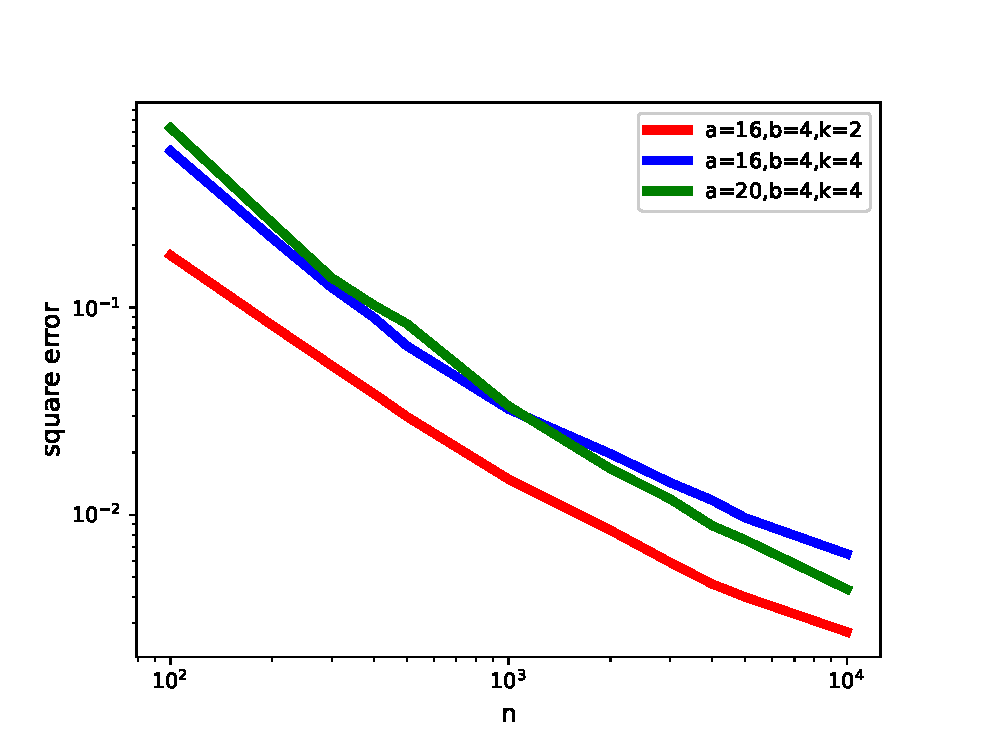
\includegraphics[width=\textwidth]{estimator-error-2020-12-20.eps}
	\caption{Estimation error of $\hat{a}, \hat{b}$ with respect to $n$.}\label{fig:estimator}
\end{subfigure}~
\begin{subfigure}{0.5\textwidth}
	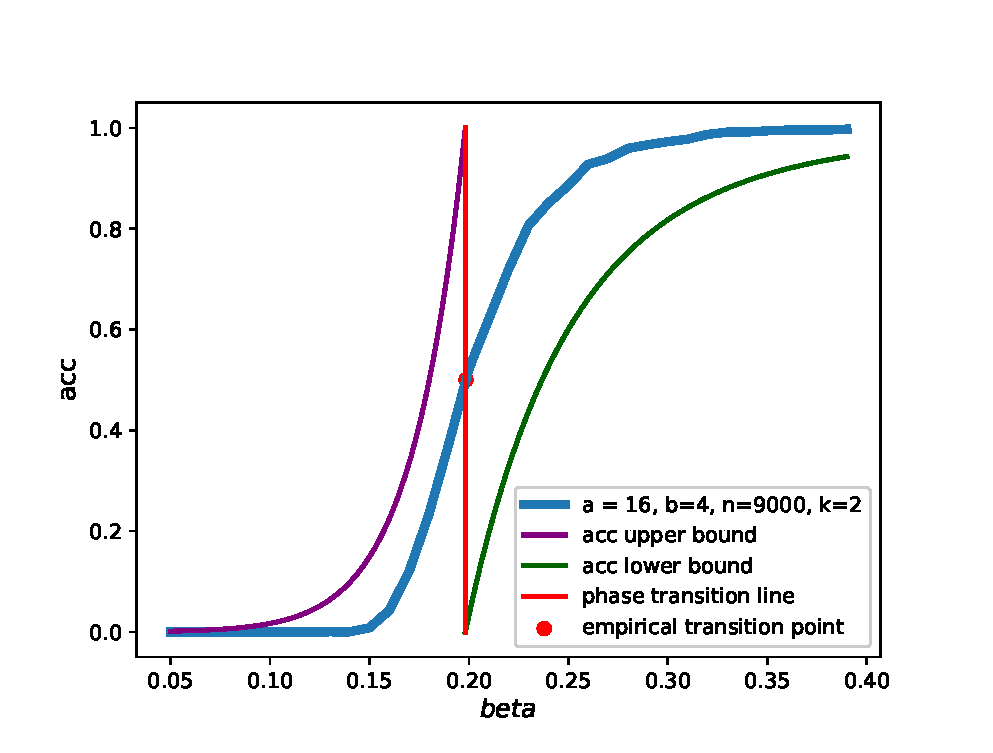
\includegraphics[width=\textwidth]{beta_trans-2020-11-28.eps}
	\caption{The accuracy of exact recovery by $\hat{X}^*$.}\label{fig:erh}
\end{subfigure}
\caption{Experimental~results.}\label{fig2}
\end{figure}
\begin{paracol}{2}
%\linenumbers
\switchcolumn


The vertical red line ($\beta=\beta^* = 0.198$), computed from \eqref{eq:beta_star}, represents the phase transition threshold. The~point $(0.199,\frac{1}{2})$ in the figure
can be regarded as the empirical phase transition threshold, whose first coordinate is close to $\beta^*$.
The green line $(\beta, n^{g(\beta)/2})$ is the theoretical lower bound of accuracy for $\beta>\beta^*$, and the purple line
$(\beta, n^{-g(\beta)})$ is the theoretical upper bound of accuracy for $\beta < \beta^*$. It can be expected that
as $n$ becomes larger, the~empirical accuracy curve (blue line in the figure) will approach the step function, which jumps from
0 to 1 at $\beta=\beta^*$.
\section{Conclusions}
In this paper, we presented  one convergent estimator (in Theorem \ref{thm:ab12}) to infer the parameters of the SBM and analyzed three label estimators to detect communities of the SBM.
We gave the exact recovery error upper bound for all label estimators (in Theorems \ref{thm:phase_transition} and \ref{thm:error_rate})
and studied their relationships. By~introducing the Ising model, our work makes a new path to study the exact recovery problem for the SBM. More
theoretical and empirical work will be done in the future, such as convergence analyses on modularity (in Equation \eqref{eq:Qtransform}), the~necessary iteration time (in Algorithm \ref{alg:m}) for Metropolis sampling, and~so~on.

\section{Proof of Main~Theorems}\label{sec:pm}
\subsection{Proof of Theorem \ref{thm:ab12}}
\begin{Lemma}\label{lem:ER_tr_counting}
	Consider an Erdős–Rényi random graph $G$ with $n$ nodes, in~which edges are placed independently with probability $p$ \cite{erdHos1960evolution}. Suppose
	$p=\A$, the~number of edges is denoted by $|E|$ while the number of triangles is $T$. Then
	$\frac{|E|}{n \log n} \to \frac{a}{2}$ and $\frac{T}{\log^3 n} \to \frac{a^3}{6}$ in probability.
\end{Lemma}
\begin{proof}
		Let $X_{ij}$ represent a Bernoulli random variable with parameter $p$. Then $|E| = \sum_{i,j} X_{ij}$, $X_{ij}$ are i.i.d.
	$\mathbb{E}[T(G)] = \frac{n(n-1)}{2}p = \frac{(n-1)\log n}{2}a$ and $\Var[|E|] = \frac{n(n-1)}{2} p(1-p) < a\frac{(n-1)\log n}{2}$.
	Then by Chebyshev's inequality,
	\begin{align*}
	P(\Big|\frac{|E|}{n \log n } - \frac{a}{2} \frac{n-1}{n}\Big| > \epsilon) & \leq
	\frac{\Var[|E| /(n \log n )]}{\epsilon^2} \\
	& < \frac{a(n-1)}{2n^2\epsilon^2\log n}
	\end{align*}
	
	For a given $\epsilon$, when $n$ is sufficiently large,
	\begin{align*}
	P(\Big|\frac{|E|}{n \log n } - \frac{a}{2} \Big| > \epsilon) & <
	P(\Big|\frac{|E|}{n \log n } - \frac{a}{2} \frac{n-1}{n}\Big| > 2\epsilon) \\
	& \leq \frac{n-1}{8n^2 \epsilon^2 \log n}
	\end{align*}
	
	Therefore, by~the definition of convergence in probability, we have $\frac{|E|}{n \log n} \to \frac{a}{2}$ as $n\to \infty$.
	
	Let $X_{ijk}$ represents a Bernoulli random variable with parameter $p^3$.
	Then $T = \sum_{i,j,k} X_{ijk}$.
	It is easy to compute that $\mathbb{E}[T] = \binom{n}{3}p^3$. Since $X_{ijk}$ are not independent, the~variance of $T$ needs careful calculation.
	From~\cite{holland1977method} we know that:
	% Mordern version: https://stats.stackexchange.com/questions/338267/distribution-and-variance-of-count-of-triangles-in-random-graph
	\begin{align*}
	\Var[T] & = \binom{n}{3} p^3 + 12 \binom{n}{4} p^5 + 30 \binom{n}{5} p^6 + 20 \binom{n}{6} p^6\\
	 &- \binom{n}{3}^2 p^6   = O(\log^3 n)
	\end{align*}
	
	Therefore
	by Chebyshev's inequality,
	\begin{align*}
	P(\Big|\frac{T}{\log^3 n } - \frac{a^3}{6} \frac{(n-1)(n-2)}{n^2}\Big| > \epsilon) &\leq \frac{\Var[T /\log^3 n ]}{\epsilon^2} \\ 
	& = \frac{1}{\epsilon^2}O(\frac{1}{\log^3 n})
	\end{align*}
	
	Hence, $\frac{T}{\log^3 n} \to \frac{a^3}{6}$.
\end{proof}
The convergence of $|E|$ in the Erdős–Rényi %define if appropriate.
graph can be extended directly to the SBM since the existence of each edge is independent.
However, for $T$, it is a little tricky since the existences of each triangle are mutually dependent. The~following two lemmas
give the formula for the variance of inter-community triangles in the SBM.
\begin{Lemma}\label{lem:SBM_tr_counting_cross}
	Consider a two-community SBM $(2n, p, q)$ and count the number of triangles $T$, which has a node in $S_1$ and an edge in $S_2$.
Then the variance of $T$ is:
\begin{align}
\Var[T] & = \frac{n^2(n-1)}{2}q^2p + n^2(n-1)(n-2)p^2q^3 \notag \\
& + \frac{n^2(n-1)^2}{2}q^4p - \frac{n^2(n-1)(3n-4)}{2}q^4 p^2 \label{eq:SBM_tr_counting_cross}
\end{align}
\end{Lemma}
\begin{Lemma}\label{lem:SBM_tr_counting_3}
	Consider a three-community SBM$(3n, p, q)$ and count the number of triangles $T$, which has a node in $S_1$, one node in $S_2$, and one node in $S_3$.
	Then the variance of $T$ is:
	\begin{equation*}\label{eq:SBM_tr_counting_three}
	\Var[T] = n^3 q^3  + 3n^3(n-1) q^4  + 3 n^3 (n-1)^2 q^5 - n^3(3n^2-3n+1)q^6
	\end{equation*}
\end{Lemma}
The proof of the above two lemmas uses some counting techniques and is similar to that in~\cite{holland1977method}, and~we omit it here.
\begin{Lemma}\label{lem:sbmV}
	For a SBM$(n, k, p, q)$ where $p=\frac{a\log n}{n}, q = \frac{b\log n}{n}$. The~number of triangles is $T$.
	Then $\frac{T}{(\log n)^3}$ converges to $\frac{1}{k^2}(\frac{a^3}{6} + \frac{k-1}{2}ab^2 + (k-1)(k-2)\frac{b^3}{6} )$ in probability as $n \to \infty$.
\end{Lemma}
\begin{proof}
	We split $T$ into three parts: the~first is the number of triangles within community $i$, $T_i$. There are $k$ terms of $T_i$.
	The second is the number of triangles that have one node in community $i$ and one edge in community $j$, $T_{ij}$. There are $k(k-1)$ terms of $T_{ij}$. The~third is the number of triangles that have one node in community $i$, one node in community $j$ and one node in community $k$.
	
	We only need to show that:
\begin{align}
	\frac{T_i}{\log ^3 n} &\to \frac{(a/k)^3}{6} \\
	\frac{T_{ij}}{\log^3 n}& \to \frac{1}{2}(a/k)(b/k)^2\\
	\frac{T_{ijk}}{\log^3 n} & \to (b/k)^3
	\end{align}
	
	The convergence of $\frac{T_i}{\log ^3 n}$ comes from Lemma \ref{lem:ER_tr_counting}.
	For $T_{ij}$ we use the conclusion from Lemma \ref{lem:SBM_tr_counting_cross}.
	We replace $n$ with $n/k$, $p=a\frac{\log n}{n}$, and $q=b\frac{\log n}{n}$ in Equation \eqref{eq:SBM_tr_counting_cross}.\linebreak
	$\Var[T_{ij}] \sim \frac{ab^2}{2k^3} \log^3 n$. Since the expectation of $\frac{T_{ij}}{\log^3 n}$ is $(n/k)\binom{n/k}{2}pq^2/(\log^3 n)
	=\frac{n-1}{2n}\frac{ab^2}{k^3}$, by~Chebyshev's inequality we can show that:
	\begin{align*}
	P( \Big|\frac{T_{ij}}{\log^3 n} - \frac{n-1}{2n}\frac{ab^2}{k^3} \Big| > \epsilon) &\leq \frac{\Var[T_{ij} / \log^3 n]}{\epsilon^2} \\
	& = \frac{1}{\epsilon^2}
	O(\frac{1}{\log^3 n})
	\end{align*}
	
	Therefore, $\frac{T_{ij}}{\log^3 n} $ converges to $\frac{1}{2}(a/k)(b/k)^2$.
	
	To prove $\frac{T_{ijk}}{\log^3 n}\to (b/k)^3$, from~Lemma \ref{lem:SBM_tr_counting_3} we can get $\Var[T_{ijk}] = O(\log^5 n)$:
	$$
	P( \Big|\frac{T_{ijk}}{\log^3 n} -\frac{b^3}{k^3} \Big| > \epsilon) \leq \frac{\Var[T_{ijk} / \log^3 n]}{\epsilon^2} = \frac{1}{\epsilon^2}
	O(\frac{1}{\log n})
	$$
\end{proof}
\begin{proof}[Proof of Theorem \ref{thm:ab12}]
	Let $e^*_1 = \frac{a+(k-1)b}{2k}$, $k^2 e^*_2 = \frac{a^3}{6} + \frac{k-1}{2}ab^2 + (k-1)(k-2)\frac{b^3}{6}$
	and\linebreak $e_1 = \frac{T_1}{n\log n}, e_2 = \frac{T_2}{\log^3 n}$.
	From Lemma \ref{lem:ER_tr_counting}, $e_1 \to e^*_1$.
	From Lemma \ref{lem:sbmV}, $e_2 \to e^*_2$ as $n\to \infty$.
	Using $x=2ke_1 - (k-1)y$, we can get:
\begin{equation}
g(y): = (k-1)(y^3 - 6 e_1 y^2 + 12 e_1^2 y) + 6 e_2 - 8 k e_1^3 = 0
\end{equation}

This equation has a unique real root since $g(y)$ is increasing on\linebreak $\mathbb{R}$:  $g'(y) = 3(k-1)(y-2e_1)^2 \geq 0 $.
Next we show that the root lies within $(0, 2e_1)$.
\begin{align*}
&\lim_{n\to \infty}g(0) =  6e^*_2 - 8k(e^*_1)^3 =-\frac{3}{k^2}(k-1)(k-2)ab^2 \\
&-\frac{3(k-1)}{k^2}a^2b - \frac{k-1}{k^2} ((k-2)-(k-1)^2)b^3 < 0 \\
&\lim_{n\to \infty}g(2e_1) = 6e^*_2 - 8(e^*_1)^3 = \frac{(k-1)(a-b)^3}{k^3} > 0
% verified with sympy
\end{align*}

Therefore, we can get a unique solution $y$ within $(0, 2e_1)$. Since $(a,b)$ is a solution for the equation array, by~the continuous property of $g(y)$, $\hat{b} \to b$ and $\hat{a} \to a$ follows.
\end{proof}
\subsection{Proof of Theorem \ref{thm:phase_transition}}\label{subsec:pt}
\begin{proof}[Proof of Lemma \ref{lem:lemmaDiff}]
	First we rewrite the energy term in \eqref{eq:energy} as:
	\begin{equation*}
	H(\bar{\sigma}) = \gamma \frac{\log n}{n} \sum_{i < j} \delta(\bar{\sigma}_i, \bar{\sigma}_j)
	- (1 + \gamma\frac{\log n}{n}) \sum_{ \{i, j\} \in E(G)} \delta(\bar{\sigma}_i, \bar{\sigma}_j)
	\end{equation*}
	
	Then calculating the energy difference term by:
	\begin{align*}
	H(\bar{\sigma}') - H(\bar{\sigma}) &= (1 + \gamma\frac{\log n}{n}) \\
	&\cdot \sum_{i \in N_r(G)} (\delta(\bar{\sigma}_r, \bar{\sigma}_i) -
	\delta(\omega^s \cdot \bar{\sigma}_r, \bar{\sigma}_i)) \\
	&+ \gamma \frac{\log n}{n}\sum_{i\neq r}
	( \delta(\omega^s \cdot \bar{\sigma}_r, \bar{\sigma}_i) -
	\delta( \bar{\sigma}_r, \bar{\sigma}_i) ) \\
	& = (1 + \gamma\frac{\log n}{n})\sum_{i \in N_r(G)} J_s(\bar{\sigma}_r, \bar{\sigma}_i) \\
	&+ \gamma \frac{\log n}{n}\sum_{i=1}^n
	( \delta(\omega^s \cdot \bar{\sigma}_r, \bar{\sigma}_i) -
	\delta( \bar{\sigma}_r, \bar{\sigma}_i) +1) \\
	&= (1+\gamma \frac{\log n}{n})\sum_{i \in N_r(G)} J_s(\bar{\sigma}_r, \bar{\sigma}_i)\\
	&+ \gamma \frac{\log n}{n} (m(\omega^s \cdot \bar{\sigma}_r)-m(\bar{\sigma}_r)+1)
	\end{align*}
\end{proof}
Before diving into the technical proof of Theorem \ref{thm:phase_transition}, we need to introduce some extra
notations. When $\bar{\sigma}'$ differs from $X$ only at position $r$, taking $\bar{\sigma}=X$ in Lemma \ref{lem:lemmaDiff}, we have:
\begin{equation}\label{eq:energy_diff}
H(\bar{\sigma}') - H(\bar{\sigma}) = (1+\gamma \frac{\log n}{n})(A^0_r - A^s_r) + \gamma\frac{\log n}{n}
\end{equation}
where $A^s_r$ is defined as $A^s_r = |\{j \in [n]\backslash \{r\}: \{j, r\} \in E(G), X_j = \omega^s \cdot X_r \}|$.
Since the existence of each edge in $G$ is independent, $A^s_r \sim \textrm{Binomial}(\frac{n}{k}, \B ) $ for $s\neq 0$
and $A^0_r \sim \textrm{Binomial}(\frac{n}{k}-1, \A )$.

% Some additional notation is needed for the proof.
For the general case, we can write:
\begin{equation}\label{eq:Hgeneral}
H(\bar{\sigma}) - H(X)=
(1 + \gamma \frac{ \log n}{n})[A_{\bar{\sigma}} - B_{\bar{\sigma}}] + \gamma\frac{ \log n}{n} N_{\bar{\sigma}}
\end{equation}
in which we use $A_{\bar{\sigma}}$ or $B_{\bar{\sigma}}$ to represent the binomial random variable with parameter $\A$ or $\B$,
respectively, and $N_{\bar{\sigma}}$ is a deterministic positive number depending on $\bar{\sigma}$ but irrelevant with the graph structure.
The following lemma gives the expression of $A_{\bar{\sigma}}, B_{\bar{\sigma}}$ and $N_{\bar{\sigma}}$:
\begin{Lemma}\label{lem:minus}
	For SSBM$(n,k,p,q)$, we assume $\bar{\sigma}$ differs from the ground truth label vector $X$ in the $|\cI|:=\Dist(\bar{\sigma}, X)$ coordinate.
	Let $I_{ij} = |\{r\in [n] | X_r = w^i, \sigma_r = w^j \}|$ for $i\neq j$ and $I_{ii} = 0$. We further denote the row sum as $I_i = \sum_{j=0}^{k-1} I_{ij}$ and
	the column sum as $I'_i = \sum_{j=0}^{k-1} I_{ji}$.
	Then:
\begin{align}
	N_{\bar{\sigma}} &= \frac{1}{2}\sum_{i=0}^{k-1} (I_i - I_i')^2 \label{eq:N_w} \\
	B_{\bar{\sigma}} & \sim \textrm{Binomial}(\frac{n}{k}|\cI| + \frac{1}{2}\sum_{i=0}^{k-1}  (-2 I'_i I_i  + I'^2_i - \sum_{j=0}^{k-1} I^2_{ji}) , q)\\
	A_{\bar{\sigma}} & \sim \textrm{Binomial}(\frac{n}{k}|\cI| - \frac{1}{2}\sum_{i=0}^{k-1}  (I^2_i + \sum_{j=0}^{k-1} I^2_{ij}), p) \label{eq:A_w}
	\end{align}
\end{Lemma}
The proof of Lemma \ref{lem:minus} is mainly composed of careful counting techniques, and~we omit it here.
When $|\cI|$ is small compared to $n$, we have the following Lemma, which is an extension of Proposition 6 in~\cite{ye2020exact}. 
\begin{Lemma}\label{lem:enhanced_fb}
	For $t\in [\frac{1}{k}(b-a), 0]$
	and $ |\cI| \le n/\sqrt{\log n}$
\begin{equation} \label{eq:upmpt}
	\begin{aligned}
	& P_G(B_{\bar{\sigma}}-A_{\bar{\sigma}}\ge t |\cI| \log n)  \\
	\le & \exp\Big(|\cI|\log n
	\Big(f_{\beta}(t) - \beta t -1	+ O(\frac{1}{\sqrt{\log n}}) \Big)\Big)
	\end{aligned}
	\end{equation}
	where $f_{\beta}(t) = \min_{s\geq 0} (g(s) - st) + \beta t \leq \tilde{g}(\beta) $.
\end{Lemma}
Corresponding to the three cases of Theorem \ref{thm:phase_transition}, we use several non-trivial lemmas to 
establish the properties of the Ising model.
\begin{Lemma}\label{lem:sigmaX}
	Let $\gamma > b$. When $\Dist(\bar{\sigma}, X) \geq \frac{n}{\sqrt{\log n}}$ and $D(\bar{\sigma}, X)$, the~event\linebreak
	$P_{\sigma | G}(\sigma = \bar{\sigma} ) > \exp(-Cn) P_{\sigma | G}(\sigma = X)$
	happens with a probability (with respect to %define is appropriate
	SSBM) less than $\exp(-\tau(\gamma,\beta) n \sqrt{\log  n} )$,
	where $C$ is an arbitrary constant and $\tau(\gamma, \beta)$
	is a positive number.
\end{Lemma}
\begin{proof}
	We denote the event $P_{\sigma | G}(\sigma = \bar{\sigma} ) > \exp(-Cn) P_{\sigma | G}(\sigma = X)$ as $\widetilde{D}(\bar{\sigma}, C)$.
	By Equation \eqref{eq:Hgeneral}, $\widetilde{D}(\bar{\sigma}, C)$
	is equivalent to:
\begin{equation}\label{eq:BwA}
	(1 + \frac{\gamma \log n}{n})[B_{\bar{\sigma}} - A_{\bar{\sigma}}] >  \frac{\gamma \log n}{n} N_{\bar{\sigma}}  - \frac{C}{\beta} n
	\end{equation}
	
	We claim that $\bar{\sigma}$ must satisfy at least one of the following two~conditions:
	\begin{enumerate}
		\item $\exists i\neq j$ s.t. $\frac{1}{k(k-1)}\frac{n}{\sqrt{\log n}} \leq I_{ij} \leq \frac{n}{k} - \frac{1}{k(k-1)}\frac{n}{\sqrt{\log n}}$
		\item $\exists i \neq j$ s.t. $I_{ij} > \frac{n}{k} - \frac{1}{k(k-1)}\frac{n}{\sqrt{\log n}}$ and $I_{ji} < \frac{1}{k(k-1)}\frac{n}{\sqrt{\log n}}$
	\end{enumerate}
	
	If neither of the above two condition holds, then from condition 1 we have\linebreak
	$I_{ij} < \frac{1}{k(k-1)}\frac{n}{\sqrt{\log n}}$ or $I_{ij} > \frac{n}{k} - \frac{1}{k(k-1)}\frac{n}{\sqrt{\log n}}$ for any $0 \leq i,j\leq k-1$.
	Since\linebreak $\sum_{i,j} I_{ij} = |\cI| \geq \frac{n}{\sqrt{\log n}}$, there exists $i,j$ such that $I_{ij} > \frac{n}{k} - \frac{1}{k(k-1)}\frac{n}{\sqrt{\log n}}$.
	Under such conditions, we also assume $I_{ji} > \frac{n}{k} - \frac{1}{k(k-1)}\frac{n}{\sqrt{\log n}}$.
	Let $X'$ be the vector that exchanges the value of $w^i$ with $w^j$ in $X$. We consider:
\begin{align}
	 \Dist(\bar{\sigma}, X') & - \Dist(\bar{\sigma}, X)= |\{ r \in [n]|X_r=w^i, \bar{\sigma}_r \neq w^j \}| \notag\\
	&+ |\{ r \in [n]|X_r=w^j, \bar{\sigma}_r \neq w^i \}| \notag\\
	&-|\{ r \in [n]|X_r=w^i, \bar{\sigma}_r \neq w^i \}| \notag\\
	&- |\{ r \in [n]|X_r=w^j, \bar{\sigma}_r \neq w^j \}| \notag\\
	& = \frac{n}{k} - I_{ij} +  \frac{n}{k} - I_{ji} - I_i - I_j\label{eq:distsmall} \\
	& < \frac{2}{k(k-1)}\frac{n}{\sqrt{\log n}} - I_i - I_j < 0\notag
	\end{align}
	which contradicts with the fact that $\bar{\sigma}$ is nearest to $X$.
	Therefore, we should have $I_{ji} < \frac{1}{k(k-1)}\frac{n}{\sqrt{\log n}}$.
	Now the $(i, j)$ pair satisfies condition 2, which contracts with the fact that $\bar{\sigma}$ satisfies neither of the two~conditions.
	
	Under condition 1, we can get a lower bound on $|A_{\bar{\sigma}}|$ from Equation \eqref{eq:A_w}. Let $I'_{ij} = I_{ij}$ for $i\neq j$ and
	$I'_{ii} = \frac{n}{k} - I_i$. Then we can simplify $|A_{\bar{\sigma}}|$ as:
	\begin{align*}
	|A_{\bar{\sigma}}| &= \frac{n}{k}|\cI| - \frac{1}{2}\sum_{i=0}^{k-1}  (I^2_i + \sum_{j=0}^{k-1} I^2_{ij}) \\
	&= \frac{n^2}{2k} - \frac{1}{2} \sum_{i=0}^{k-1} \sum_{j=0}^{k-1} I'^2_{ij}
	\end{align*}
	
	We further have $\sum_{i=0}^{k-1} \sum_{j=0}^{k-1} I'^2_{ij} \leq (k-1)\frac{n^2}{k^2} + (\frac{n}{k} - I_{ij})^2 + I^2_{ij}$ where
	$I_{ij}$ satisfies condition 1. Therefore, $\sum_{i=0}^{k-1} \sum_{j=0}^{k-1} I'^2_{ij} \leq (k-1)\frac{n^2}{k^2} + (\frac{1}{k(k-1)}\frac{n}{\sqrt{\log n}})^2
	+ (\frac{n}{k} - \frac{1}{k(k-1)}\frac{n}{\sqrt{\log n}})^2 = \frac{n^2}{k} - \frac{2n^2}{k^2 (k-1)\sqrt{\log n}}(1+o(1))$.
	As a result,
\begin{equation}\label{eq:Asigma}
	A_{\bar{\sigma}} \geq \frac{n^2}{k^2 (k-1)\sqrt{\log n}}(1+o(1))
	\end{equation}
	
	
	Under condition 2, we can get a lower bound on $N_{\bar{\sigma}}$. Since
	$\Dist(\bar{\sigma}, X') - \Dist(\bar{\sigma}, X) \geq 0$, from~\eqref{eq:distsmall} we have
	$I_{ij} + I_{ji} + I_{i} + I_j \leq \frac{2n}{k} $.
	Since $I_i \geq I_{ij} > \frac{n}{k} - \frac{1}{k(k-1)}\frac{n}{\sqrt{\log n}}$,
	we have\linebreak $I_j \leq \frac{2}{k(k-1)}\frac{n}{\sqrt{\log n} }$.
	Now consider $I'_j - I_j \geq  \frac{n}{k} - \frac{3}{k(k-1)}\frac{n}{\sqrt{\log n} }$.
	From \eqref{eq:N_w}:\linebreak $N_{\bar{\sigma}} \geq \frac{1}{2}(\frac{n}{k} - \frac{3}{k(k-1)}\frac{n}{\sqrt{\log n}})^2 = \frac{n^2}{2k^2}(1+o(1))$.
	
	Now we use the Chernoff inequality to bound Equation \eqref{eq:BwA}; we can omit $\frac{\gamma \log n}{n}$ on the left-hand side since it is far smaller than $1$.
	Let $Z \sim \textrm{Bernoulli}(\A), Z' \sim \textrm{Bernoulli}(\B)$, then:
	\begin{align*}
	&P_G(\widetilde{D}(\bar{\sigma}, C))
	\leq (\mathbb{E}[\exp(sZ')])^{|B_{\bar{\sigma}}|}(\mathbb{E}[\exp(-sZ)])^{|A_{\bar{\sigma}}|}\\
	&\cdot \exp(-s(\frac{\gamma \log n}{n} N_{\bar{\sigma}}  - \frac{C}{\beta}n)) \\
	& \leq \exp\Big(|B_{\bar{\sigma}}|\frac{b\log n}{n}(e^s -1) + |A_{\bar{\sigma}}|\frac{a\log n}{n} (e^{-s} - 1) \\
	&-s(\frac{\gamma \log n}{n} N_{\bar{\sigma}}  - \frac{C}{\beta}n)\Big) 
	\end{align*}
	
	Using $|B_{\bar{\sigma}}| = N_{\bar{\sigma}} + |A_{\bar{\sigma}}|$ we can further simplify the exponential term as:
	$$
	\frac{\log n}{n} [|A_{\bar{\sigma}}|(b(e^s -1)+ a(e^{-s} - 1)) +
	N_{\bar{\sigma}} (b(e^s - 1)-\gamma s)]  + s \frac{C}{\beta}n
	$$
	
	Now we investigate the function $g_1(s) = b(e^s -1)+ a(e^{-s} - 1)$ and\linebreak $g_2(s) = b(e^s - 1)-\gamma s$.
	Both functions take zero values at $s=0$ and\linebreak $g_1'(s) = (be^s - ae^{-s}), g_2'(s) = be^s -\gamma$.
	Therefore, $g_1'(0) = b-a<0, g_2'(0) = b - \gamma < 0$ and we can choose $s^*>0$ such that $g_1(s^*) < 0,g_2(s^*) < 0$.
	To compensate the influence of the term $sCn/\beta$ we only need to make sure that the order of $\frac{\log n}{n} \min\{|A_{\bar{\sigma}}|, N_{\bar{\sigma}}\}$ is larger than $n$.
	This requirement is satisfied since either $|A_{\bar{\sigma}}|\geq \frac{n^2}{k^2 (k-1)\sqrt{\log n}}(1+o(1))$ or $N_{\bar{\sigma}} \geq \frac{n^2}{2k^2}(1+o(1))$.
\end{proof}
\begin{Lemma}\label{prop:small}
	If $\gamma>b$, $\beta>\beta^\ast$,
	For $1\leq r \leq \frac{n}{\sqrt{\log n}}$
	and $\forall \epsilon > 0$, there is a set $\cG^{(r)}$ such that:
\begin{equation}\label{eq:Gr}
	P_G(\cG^{(r)}_n) \ge 1 - n^{r(\tilde{g}(\beta)/2 + \epsilon)}
	\end{equation}
	and
	for every $G\in\cG^{(r)}_n$,
\begin{equation}\label{eq:psigmaX}
	\frac{P_{\sigma|G}(\Dist(\sigma, X)=r | D(\sigma, X))}
	{P_{\sigma|G}(\sigma=X | D(\sigma, X))} <
	n^{r \tilde{g}(\beta) /2}
	\end{equation}
	
	For $r> \frac{n}{\sqrt{\log n}}$, there is a set $\cG^{(r)}$ such that:
\begin{equation}\label{eq:Gr1}
	P(G\in\cG^{(r)}_n) \ge 1 - e^{-n}
	\end{equation}
	and
	for every $G\in\cG^{(r)}_n$,
\begin{equation}\label{eq:psigmaX1}
	\frac{P_{\sigma|G}(\Dist(\sigma, X)=r | D(\sigma, X))}
	{P_{\sigma|G}(\sigma=X | D(\sigma, X))} <
	e^{-n}
	\end{equation}
\end{Lemma}


\begin{proof}
We distinguish the discussion between two cases: $r\leq \frac{n}{\sqrt{\log n}}$
and $r > \frac{n}{\sqrt{\log n}}$.

When $r\leq \frac{n}{\sqrt{\log n}}$, we can show that $\Dist(\sigma, X) = r$ implies $D(\sigma, X)$ by using the triangle
inequality of $\Dist$. For~$f \in S_k \backslash \{ \textrm{id} \}$, where $\textrm{id}$ is the identity mapping, we have:
$$
\frac{2n}{k} \leq \Dist(f(X), X) \leq \Dist(\sigma, f(X)) + \Dist(\sigma, X)
$$

Therefore, $\Dist(\sigma, f(X)) \geq \frac{2n}{k} - \frac{n}{\sqrt{\log n}} \geq \Dist(\sigma, X)$ and Equation
\eqref{eq:psigmaX} is equivalent with:
\begin{equation}\label{eq:psigmaX2}
\frac{P_{\sigma|G}(\Dist(\sigma, X)=r)}
{P_{\sigma|G}(\sigma=X)} <
n^{r \tilde{g}(\beta) /2}
\end{equation}

The left-hand side can be written as:
\begin{align*}
\frac{P_{\sigma|G}(\Dist(\sigma, X)=r)}
{P_{\sigma|G}(\sigma=X)}  &= \sum_{\Dist(\bar{\sigma}, X)=r}\exp(-\beta(H(\bar{\sigma})-H(X)))\\
\textrm{ by \eqref{eq:Hgeneral} } &\leq \sum_{\Dist(\bar{\sigma}, X)=r}\exp(\beta_n(B_{\bar{\sigma}}-A_{\bar{\sigma}}))
\end{align*}
where $\beta_n = \beta(1+\gamma\frac{\log n}{n})$.

Define $\Xi_n(r): = \sum_{\Dist(\bar{\sigma}, X)=r}\exp(\beta_n(B_{\bar{\sigma}}-A_{\bar{\sigma}}))$ and we only need to show that:
\begin{equation}
P_{G}(\Xi_n(r) \geq n^{r \tilde{g}(\beta) /2}) \leq  n^{r (\tilde{g}(\beta) /2 + \epsilon)}
\end{equation}

Define the event $\Lambda_n(G,r):=\{B_{\bar{\sigma}} -A_{\bar{\sigma}} < 0, \forall \bar{\sigma}\, s.t. \Dist(\bar{\sigma}, X)=r\}$,
and we proceed as~follows:
\begin{align*}
P_{G}(\Xi_n(r) \geq n^{r \tilde{g}(\beta) /2}) &\leq
P_G(\Lambda_n(G,r)^c) \\
&+ P_G(\Xi_n(r) \geq n^{r \tilde{g}(\beta) /2} |\Lambda_n(G,r) )
\end{align*}

For the first term, since $|\{ \bar{\sigma} | \Dist(\bar{\sigma}, X) = r \}|  \leq (k-1)^r n^r$,
by Lemma \ref{lem:enhanced_fb},\linebreak
$P_G(\Lambda_n(G,r)^c) \leq (k-1)^r n^{rg(\bar{\beta})} \leq n^{r (\tilde{g}(\beta) /2 + \epsilon/2)}$.
For the second term, we use Markov~inequality:
\begin{align*}
P_G(\Xi_n(r) \geq n^{r \tilde{g}(\beta) /2} |\Lambda_n(G,r) )
\leq \mathbb{E}[\Xi_n(r)|\Lambda_n(G,r)]n^{-r \tilde{g}(\beta) /2} 
\end{align*}

The conditional expectation can be estimated as follows:
\begin{align*}
&\mathbb{E}[\Xi_n(r)|\Lambda_n(G,r)]=
\sum_{\Dist(\bar{\sigma}, X) = r}\sum_{tr\log n = -\infty }^{-1} \\
& P_G(B_{\bar{\sigma}} -A_{\bar{\sigma}}=tr\log n)\exp(\beta_n tr \log n) \\
& \leq (k-1)^r n^{r+r\beta_n(b-a)/k} +
\sum_{\Dist(\bar{\sigma}, X) = r}\sum_{tr\log n = r\frac{b-a}{k}\log n }^{-1} \\
& P_G(B_{\bar{\sigma}} -A_{\bar{\sigma}}=tr\log n)\exp(\beta_n tr \log n)
\end{align*}
$1+\beta_n(b-a)/k = f_{\beta_n}(\frac{b-a}{k}) < \tilde{g}(\beta_n)$, therefore,
$(k-1)^r n^{r+r\beta_n (b-a)/k}n^{-r \tilde{g}(\beta) /2} \leq$\linebreak $n^{r (\tilde{g}(\beta) /2 + \epsilon/2)} $.
Using Lemma \ref{lem:enhanced_fb}, we have:
\begin{align*}
P_G(B_{\bar{\sigma}} -A_{\bar{\sigma}}=tr\log n)\exp(\beta_n rt \log n) \leq 
n^{r(f_{\beta_n}(t)-1 + O(\frac{1}{\sqrt{\log n}}))}
\end{align*}

Since $\beta_n \to \beta$, $\forall \epsilon$, when $n$ is sufficiently large
we have $\tilde{g}(\beta_n) \leq \tilde{g}(\beta) + \epsilon /2$.
Therefore,
\begin{align*}
&n^{-r \tilde{g}(\beta) /2}\sum_{\Dist(\bar{\sigma}, X) = r}\sum_{\substack{tr\log n = \\ r(b-a)/k\log n} }^{-1}
P_G(B_{\bar{\sigma}} -A_{\bar{\sigma}}=t\log n)\exp(\beta_n rt \log n) \\
& \leq  (k-1)^r r\frac{b-a}{k} ( \log n ) n^{r(\tilde{g}(\beta_n) - \tilde{g}(\beta)/2)}\\
& \leq  n^{r(\tilde{g}(\beta)/2 + \epsilon/2)} O(\log n) (k-1)^r
\end{align*}

Combining the above equations, we have:
\begin{align*}
P_{G}(\Xi_n(r) \geq n^{r \tilde{g}(\beta) /2}) &\leq  n^{r(\tilde{g}(\beta)/2 + \epsilon/2)} O(\log n) (k-1)^r\\
&\leq n^{r(\tilde{g}(\beta)/2 + \epsilon)}
\end{align*}

When $r>\frac{n}{\sqrt{\log n}}$, using Lemma \ref{lem:sigmaX}, we can choose a sufficiently large constant $C>1$
such that $k^n\exp(-Cn) < e^{-n}$:
\begin{align*}
\frac{P_{\sigma|G}(\Dist(\sigma, X)=r | D(\sigma, X))}
{P_{\sigma|G}(\sigma=X | D(\sigma, X))} &= \sum_{\substack{D(\bar{\sigma}, X) \\ \Dist(\bar{\sigma}, X)=r}}
\frac{P_{\sigma | G}(\sigma = \bar{\sigma}) }{P_{\sigma | X}(\sigma = X)} \\
&> \exp(-n)
\end{align*}
happens with probability less than $e^{-n}$. Therefore,  Equation \eqref{eq:psigmaX1} holds.
\end{proof}

If $\gamma > b$ and $\beta < \beta^*$, we have the following lemma:
\begin{Lemma}\label{lem:7}
	If $\gamma > b$ and $\beta < \beta^*$, there is a set $\cG^{(1)}_n$ such that
	$P_G(\cG^{(1)}_n) \geq 1-n^{g(\bar{\beta})}$
	and:
\begin{align}
	\mathbb{E}[\sum_{r=1}^n \exp(\beta_n (A_r^s - A_r^0)) | G \in \cG^{(1)}_n] &= (1+o(1))n^{g(\beta_n)} \\
	\Var[\sum_{r=1}^n \exp(\beta_n (A_r^s - A_r^0)) | G \in \cG^{(1)}_n] &\leq n^{g(\beta_n)}
	\end{align}
\end{Lemma}
Lemma \ref{lem:7} is an extension of Proposition 10 in~\cite{ye2020exact} and can be proved using almost the same analysis. Thus we omit the
proof of Lemma \ref{lem:7} here.
\begin{Lemma}\label{prop:large2}
	If $\gamma > b$ and $\beta < \beta^*$, there is a set $\cG'_n$ such that:
\begin{equation}
	P_G(\cG'_n) \geq 1 - (1+o(1))\max\{n^{g(\bar{\beta})}, n^{ - g(\beta_n) + \epsilon} \}
	\end{equation}
	and for every $G \in \cG'_n$,
\begin{equation}\label{eq:diff1g}
	\frac{P_{\sigma|G}(\Dist(\sigma, X)=1 | D(\sigma, X))}
	{P_{\sigma|G}(\sigma=X | D(\sigma, X))} \geq (k-1+o(1))n^{g(\beta_n)}
	\end{equation}
	
\end{Lemma}
\begin{proof}
The left-hand side of Equation \eqref{eq:diff1g} can be rewritten as:
\begin{equation}\label{eq:knd}
	\frac{P_{\sigma|G}(\Dist(\sigma, X)=1)}
{P_{\sigma|G}(\sigma=X)}= (1+o(1))\sum_{s=1}^{k-1}\sum_{r=1}^n \exp(\beta_n (A_r^s - A_r^0))
\end{equation}

Let $\cG^{(1)}_n$ be defined in Lemma \ref{lem:7}
and $\cG^{(2)}_n: = \{|\sum_{r=1}^n \exp(\beta_n (A_r^s - A_r^0)) -\linebreak (1+o(1))n^{g(\beta_n)}  | \leq n^{g(\beta_n) - \epsilon / 2} \}$.

Using Chebyshev's inequality, we have:
\begin{equation*}
P_G(G \not\in \cG^{(2)}_n \Big\vert  G \in \cG^{(1)}_n) \leq n^{- g(\beta_n) + \epsilon}
\end{equation*}

Let $\cG'_n = \cG^{(1)}_n \cap \cG^{(2)}_n$:
\begin{align*}
P_G(G \in \cG'_n) &= P_G(\cG^{(1)}_n) P_G(G \in \cG_n^{(2)} | G \in \cG_n^{(1)}) \\
& \geq (1-n^{ - g(\beta_n) + \epsilon})(1-n^{g(\bar{\beta})}) \\
&= 1-(1+o(1))\max\{n^{g(\bar{\beta})}, n^{- g(\beta_n) + \epsilon} \}
\end{align*}
and for every $G\in\cG'_n$,
\begin{equation*}
\sum_{r=1}^n \exp(\beta_n (A_r^s - A_r^0)) = (1+o(1)) n^{g(\beta_n)}
\end{equation*}

Therefore, from Equation~\eqref{eq:knd} we have:
\begin{equation*}
	\frac{P_{\sigma|G}(\Dist(\sigma, X)=1)}
{P_{\sigma|G}(\sigma=X)} \geq (k-1+o(1)) n^{g(\beta_n)}
\end{equation*}
\end{proof}

Let $\Lambda := \{ \omega^j  \cdot \mathbf{1}_n | j=0, \dots,k-1\}$
where $\mathbf{1}_n$ is the all-ones vector %confirm.
 with dimension $n$, and~we have the following lemma:
\begin{Lemma}\label{lem:small}
	Suppose $\gamma < b $ and $\bar{\sigma}$ satisfies $\Dist(\bar{\sigma}, \mathbf{1}_n) \geq \frac{n}{\sqrt{\log  n}}$
	and $D(\bar{\sigma}, \mathbf{1}_n)$.
	Then the event
	$P_{\sigma | G}(\sigma = \bar{\sigma} ) > \exp(-Cn) P_{\sigma | G}(\sigma = \mathbf{1}_n)$
	happens with a probability (with respect to SSBM) less than $\exp(-\tau(\gamma,\beta) n \sqrt{\log  n} )$ where $C$ is an arbitrary constant, $\tau(\gamma,\beta)$ is a positive number.
\end{Lemma}
\begin{proof}
	Let $n_r = |\{\bar{\sigma}_i = w^r | i\in [n] \}|$. Then $n_0 \geq n_r$ for $r=1, \dots, k-1$ since\linebreak $\arg\,\min_{\sigma'\in \Lambda} \Dist(\bar{\sigma}, \sigma') = \mathbf{1}_n$.
	Without loss of generality,
	we suppose \mbox{$n_0 \geq n_1 \dots \geq n_{k-1}$}.
	Define $N_{\bar{\sigma}} = \frac{1}{2}(n(n-1) - \sum_{r=0}^{k-1} n_r(n_r-1))
	=\frac{1}{2}(n^2 - \sum_{r=0}^{k-1} n_r^2)$.
	Denote the event\linebreak $P_{\sigma | G}(\sigma = \bar{\sigma} ) > \exp(-Cn) P_{\sigma | G}(\sigma = \mathbf{1}_n)$ as $D'(\bar{\sigma}, C)$,
	which can be transformed as:
\begin{align}
	(1 + \frac{\gamma \log n}{n})
	\left( \sum_{\bar{\sigma}_i  \neq \bar{\sigma}_j, X_i = X_j} Z_{ij} +
	\sum_{\bar{\sigma}_i  \neq \bar{\sigma}_j, X_i \neq X_j} Z_{ij} \right)\notag\\
	\leq \frac{\gamma \log n}{n} N_{\bar{\sigma}} + \frac{C}{\beta} n\label{eq:small}
	\end{align}
		
	Firstly we estimate the order of $N_{\bar{\sigma}}$, and obviously $N_{\bar{\sigma}} \leq \frac{1}{2} n^2$.
	Using the conclusion in Appendix A of~\cite{chen2016information}, we have:
\begin{equation}
	\sum_{r=0}^{k-1} n_r^2 \leq
	\begin{cases}
	n n_0 & n_0 \leq \frac{n}{2} \\
	n^2 - 2n_0(n-n_0) & n_0 > \frac{n}{2}
	\end{cases}
	\end{equation}
	
	By assumption of $\Dist(\bar{\sigma}, \mathbf{1}_n) \geq \frac{n}{\sqrt{\log n}}$, we have $n_0 \leq n - \frac{n}{\sqrt{\log n}}$
	and $n_0 \geq \frac{n}{k}$ follows from $n_0 \geq n_r$.
	When $n_0 > \frac{n}{2}$,
	we have $N_{\bar{\sigma}} \geq n_0 (n - n_0) \geq \frac{n^2}{\sqrt{\log n}}(1+o(1))$.
	The second inequality is achieved if $n_0 = n - \frac{n}{\sqrt{\log n}}$.
	When $n_0 < \frac{n}{2}$,
	$N_{\bar{\sigma}} \geq \frac{n^2 - nn_0}{2} \geq \frac{n^2}{4}$ and the second inequality is achieved when $n_0 = \frac{n}{2}$.
	Thus generally we have $\frac{n^2}{\sqrt{\log n}}(1+o(1)) \leq N_{\bar{\sigma}} \leq \frac{n^2}{2}$.
	
	Since $\frac{C}{\beta} n = o(\frac{\log n}{n} N_{\bar{\sigma}})$ we can rewrite Equation \eqref{eq:small} as:
\begin{equation}
	\left( \sum_{\substack{\bar{\sigma}_i  \neq \bar{\sigma}_j \\ X_i = X_j}} -Z_{ij}
	+ \sum_{\substack{\bar{\sigma}_i  \neq \bar{\sigma}_j \\ X_i \neq X_j}} -Z_{ij} \right)\geq -\gamma\frac{\log n N_{\bar{\sigma}}}{n}(1+o(1))
	\end{equation}
	
	Let $N_1 = \sum_{\bar{\sigma}_i  \neq \bar{\sigma}_j, X_i = X_j} 1$
	and $N_2 = \sum_{\bar{\sigma}_i  \neq \bar{\sigma}_j, X_i \neq X_j} 1 = N_{\bar{\sigma}} - N_1$.
	
	Using the Chernoff inequality we have:
	\begin{align*}
	P_G(D'(\bar{\sigma}, C))&
	\leq (\mathbb{E}[\exp(-s Z )])^{N_1} (\mathbb{E}[\exp(-s Z' )])^{N_2} \\
	&\cdot \exp(\gamma \frac{\log n N_{\bar{\sigma}} s}{n}(1+o(1))) \\
	&= \exp \Big( \frac{\log n}{n}(1+o(1))(e^{-s}-1)(aN_1 + bN_2) \\
	&+\gamma \frac{\log n N_{\bar{\sigma}} s}{n}(1+o(1))\Big)
	\end{align*}
	
	Since $s > 0$ and $a>b$, we further have:
	\begin{align*}
	P_G(D'(\bar{\sigma}, C))
	& \leq \exp( \frac{N_{\bar{\sigma}}\log n }{n}(b(e^{-s}-1)+ \gamma s + o(1))) 
	\end{align*}
	
	Let $h_b(x) = x - b -x\log \frac{x}{b}$, which satisfies $h_b(x) < 0$ for $0<x<b$,
	and take $s=-\log\frac{\gamma}{b} > 0$, using 
	$N_{\bar{\sigma}} \geq \frac{n^2}{\sqrt{\log n}}$ we have:
	\begin{align*}
	P_G(D'(\bar{\sigma}, C))&\leq \exp( N_{\bar{\sigma}} \frac{\log n}{n} h_b(\gamma)(1+o(1))) \\
	& \leq \exp (h_b(\gamma) n \sqrt{\log n} (1+o(1)))
	\end{align*}
\end{proof}
\begin{proof}[Proof of Theorem \ref{thm:phase_transition}]
	(1) Since $P_{\sigma}(\sigma \not \in S_k(X)) = \sum_{f\in S_k} P_{\sigma}(\sigma \neq f(X) | D(\sigma, f(X)))\linebreak P_{\sigma}(D(\sigma, f(X)))$,
	we only need to establish $P_{\sigma}(\sigma \neq X | D(\sigma, X)) \leq  n^{\tilde{g}(\beta)/2 + \epsilon}$.
	From \mbox{Lemma \ref{prop:small}}, we can find $\cG_n^{(r)}$ for $r=1,\dots, n$.
	Let $\cG'_n = \cap_{r=1}^n \cG_n^{(r)}$ and choose $\frac{\epsilon}{2}$; from Equations~(\ref{eq:Gr}) and (\ref{eq:Gr1}), we~have:
	\begin{align*}
	P_G(\cG'^c_n) &= P_G(\cup_{r=1}^n (\cG_n^{(r)})^c) \\
	&\leq \sum_{r=1}^{n/\sqrt{\log n } } n^{r(\tilde{g}(\beta)/2 + \epsilon/2)}  + n e^{-n} \\
	& \leq \frac{1}{2} n^{\tilde{g}(\beta)/2 + \epsilon}
	\end{align*}
	where the last inequality follows from the estimation of sum of geometric series.
	On the other hand, for~every $G \in \cG'_n$, from Equations~(\ref{eq:psigmaX}) and (\ref{eq:psigmaX1}),
	we have:
	\begin{align*}
	\frac{P_{\sigma | G}(\sigma \neq X | D(\sigma, X))}{1-P_{\sigma | G}(\sigma \neq X | D(\sigma, X))} &= \frac{P_{\sigma | G}(\sigma \neq X | D(\sigma, X))}{P_{\sigma|G}(\sigma=X | D(\sigma, X))} \\
	&< \sum_{r=1}^{n/\sqrt{\log n }}  n^{r\tilde{g}(\beta)/2} + n e^{-n}
	\end{align*}
	from which we can get the estimation $P_{\sigma | G}(\sigma \neq X | D(\sigma, X))\leq \frac{1}{2}n^{\tilde{g}(\beta)/2 + \epsilon}$.
	Finally, 
	\begin{align*}
	P_{\sigma}(\sigma \neq X|D(\sigma, X)) &= \sum_{G\in \cG'_n} P_G(G)P_{\sigma |G}(\sigma \neq X | D(\sigma, X)) \\
	+ P_G(\cG'^c_n)
	& \leq n^{\tilde{g}(\beta)/2 + \epsilon}.
	\end{align*}
	
	(2) When $\beta < \beta^*$, using Lemma \ref{prop:large2}, for~every $G \in \cG'_n$
	we can obtain:
	$$
	\frac{1-P_{\sigma | G}(\sigma=X | D(\sigma, X))}{P_{\sigma | G}(\sigma=X | D(\sigma, X))}\geq (k-1+o(1))n^{g(\beta_n)}
	$$
	
	We then have:
	$$
	P_{\sigma | G}(\sigma=X| D(\sigma, X)) \leq \left(\frac{1}{k-1}+o(1) \right) n^{-g(\beta_n)}
	$$
	
	Then:
	\begin{align*}
	&P_{\sigma}(\sigma=X| D(\sigma, X))  \leq  P(\cG'^c_n) \\
	&+ \sum_{G\in \cG'_n}P_G(G) P_{\sigma|G}(\sigma=X| D(\sigma, X)) \\
	& \leq (\frac{1}{k-1}+o(1))n^{-g(\beta_n)} + (1+o(1)) \max\{n^{g(\bar{\beta})}, n^{- g(\beta_n) + \epsilon} \}\\
	& \leq (1+o(1)) \max\{n^{g(\bar{\beta})}, n^{-g(\beta) + \epsilon}  \}
	\end{align*}
	
	(3) When $\gamma < b$, for~any $f\in S_k$, we have $\Dist(f(X), \Lambda) = \frac{(k-1)n}{k} > \frac{n}{\sqrt{\log n}}$.
	Therefore, using Lemma \ref{lem:small}, we can find a set $\cG'_n$ such that $P_G(\cG'_n) \leq \exp(-nC)$
	and for any $G\not \in \cG'_n$, $P_{\sigma |G}(\sigma = f(X)) \leq \exp(-Cn)$. Therefore,
	\begin{align*}
	P_a(\hat{X}^*) \leq P_G(\cG'_n) + k! \exp(-Cn) = (1+k!)\exp(-Cn)
	\end{align*}
	
	The conclusion of $P_a(\hat{X}^*) \leq \exp(-Cn)$ follows since $C$ can take any positive value.
\end{proof}

\subsection{Proof of Theorem \ref{thm:error_rate}}


\begin{Lemma}[Lemma 8 of~\cite{abbe2015exact}]\label{lem:mZW}
	Let $m$ be a positive number larger than $n$.
	When $Z_1, \dots, Z_m$ are i.i.d. Bernoulli($\B$) and $W_1, \dots, W_m$ are i.i.d Bernoulli($\A$), independent of $Z_1, \dots, Z_m$,
	then:
\begin{equation}
	P(\sum_{i=1}^m (Z_i  - W_i) \geq 0) \leq \exp(-\frac{m \log n}{n}(\sqrt{a} - \sqrt{b})^2)
	\end{equation}
\end{Lemma}
\begin{proof}[Proof of Theorem \ref{thm:error_rate}]

	Let $P_F^{(r)}$ denote the probability when there is $\sigma$ satisfying\linebreak $\Dist(\sigma, X) = r$ and $H(\sigma) < H(X)$.
	
	From Equation \eqref{eq:energy_diff}, when $\sigma$ differs from $X$ only by one coordinate, from~Lemma \ref{lem:mZW} the probability for $H(\sigma) < H(X)$ is
	bounded by $P_G(A_r^s - A_r^0 > 0) \leq n^{-\frac{(\sqrt{a}-\sqrt{b})^2}{k}}$. Therefore, $P_F^{(1)}  \leq (k-1)n^{g(\bar{\beta})}$.
	Using Lemma \ref{lem:enhanced_fb}, we can get $P_F^{(r)} \leq (k-1)^r n^{rg(\bar{\beta})}$ for $ r \leq \frac{n}{\sqrt{\log n}}$.
	For $ r \geq \frac{n}{\sqrt{\log n}}$, choosing $C=0$ in Lemma \ref{lem:sigmaX} we can get $\sum_{r\geq \frac{n}{\sqrt{\log n}}}P_F^{(r)} \leq e^{-n}$.
	That is, the~dominant term is $\sum_{r\leq \frac{n}{\sqrt{\log n}}}P_F^{(r)}$ since the other part decreases exponentially fast.
	Therefore, the~upper bound for error rate of $\hat{X}'$ is:
	\begin{align*}
	P_F = & \sum_{r=1}^n P_F^{(r)} \leq (1+o(1)) \sum_{r=1}^{\infty} (k-1)^r n^{rg(\bar{\beta})}\\
	\leq & (1+o(1))\frac{(k-1) n^{g(\bar{\beta})}}{1-(k-1) n^{g(\bar{\beta})}} = (k-1+o(1))n^{g(\bar{\beta})}
	\end{align*}
	
When $\sigma \in W^*$, since $|\{r\in [n] | \sigma_r = \omega^i \}| = I'_i + \frac{n}{k} - I_i $, we have $I'_i = I_i$.
From \mbox{Lemma \ref{lem:minus}}, we can see  $|B_{\bar{\sigma}}| = |A_{\bar{\sigma}}|$
and $N_{\bar{\sigma}} = 0$. Then from Equation \eqref{eq:Hgeneral}, $H(\bar{\sigma}) < H(X)$ is equivalent with $B_{\bar{\sigma}} > A_{\bar{\sigma}}$.

Therefore, when $ \Dist(\bar{\sigma}, X) \geq \frac{n}{\sqrt{\log n} }$ and $D(\sigma, X)$,
from Equation \eqref{eq:Asigma}, we have\linebreak $A_{\bar{\sigma}} \geq \frac{n^2}{k^2(k-1)\sqrt{\log n} } (1+o(1))$.
We use Lemma \ref{lem:mZW} by letting $m=|A_{\bar{\sigma}}|$ when $m \geq \frac{n}{ \sqrt{\log n}}$; the~error term is bounded
by $\sum_{r\geq \frac{n}{ \sqrt{\log n}}} P_F^{(r)} \leq \sum_{r\geq \frac{n}{ \sqrt{\log n}}} (k-1)^r \exp(-\frac{(\sqrt{a} - \sqrt{b})^2}{k^2(k-1)} n \sqrt{\log n}))
\leq \exp(-n)$, which decreases exponentially fast.
For $m < \frac{n}{ \sqrt{\log n}}$, we can use Lemma \ref{lem:enhanced_fb} directly 
by considering $\sum_{r=2}^{\frac{n}{ \sqrt{\log n}}} P_F^{(r)}$. The~summation starts from $r=2$ since $\sigma \in W^*$.
Therefore,
\begin{align*}
P_F = & \sum_{r=2}^n P_F^{(r)} \leq (1+o(1)) \sum_{r=2}^{\infty} (k-1)^r n^{rg(\bar{\beta})}\\
\leq & ((k-1)^2+o(1))n^{2g(\bar{\beta})}
\end{align*}
\end{proof}

%%%%%%%%%%%%%%%%%%%%%%%%%%%%%%%%%%%%%%%%%%
%\section{Patents}
%This section is not mandatory, but may be added if there are patents resulting from the work reported in this manuscript.

%%%%%%%%%%%%%%%%%%%%%%%%%%%%%%%%%%%%%%%%%%
%\vspace{6pt} 

%%%%%%%%%%%%%%%%%%%%%%%%%%%%%%%%%%%%%%%%%%
%% optional
%\supplementary{The following are available online at \linksupplementary{s1}, Figure S1: title, Table S1: title, Video S1: title.}

% Only for the journal Methods and Protocols:
% If you wish to submit a video article, please do so with any other supplementary material.
% \supplementary{The following are available at \linksupplementary{s1}, Figure S1: title, Table S1: title, Video S1: title. A supporting video article is available at doi: link.}

%%%%%%%%%%%%%%%%%%%%%%%%%%%%%%%%%%%%%%%%%%
\authorcontributions{The work of this paper was conceptualized by M.Y., who also developed the mathematical analysis methodology for the proof of the main
	theorem of this paper. All simulation code was written by F.Z., who also extended the idea of M.Y., concreted the proof and wrote this paper.
	The work is supervised and funded by S.-L.H. All authors have read and agreed to the published version of the~manuscript.}

%%%%%%%%%%%%%%%%%%%%%%%%%%%%%%%%%%%%%%%%%%
\funding{
	This research was supported in part by the Natural Science Foundation of China under Grant 61807021, in~part by the Shenzhen Science and Technology Program under Grant KQTD20170810150821146, and~in part by the Innovation and Entrepreneurship Project for Overseas High-Level Talents of Shenzhen under Grant~KQJSCX20180327144037831.
}



\institutionalreview{Not applicable}
%MDPI: In this section, please add the Institutional Review Board Statement and approval number for studies involving humans or animals. Please note that the Editorial Office might ask you for further information. Please add “The study was conducted according to the guidelines of the Declaration of Helsinki, and approved by the Institutional Review Board (or Ethics Committee) of NAME OF INSTITUTE (protocol code XXX and date of approval).” OR “Ethical review and approval were waived for this study, due to REASON (please provide a detailed justification).” OR “Not applicable” for studies not involving humans or animals. You might also choose to ex-clude this statement if the study did not involve humans or animals.

\informedconsent{Not applicable}
%MDPI: Any research article describing a study involving humans should contain this statement. Please add “Informed consent was obtained from all subjects involved in the study.” OR “Patient con-sent was waived due to REASON (please provide a detailed justification).” OR “Not applicable” for studies not involving humans. You might also choose to exclude this statement if the study did not involve humans. Written informed consent for publication must be obtained from participating patients who can be identified (including by the patients themselves). Please state “Written informed consent has been obtained from the patient(s) to publish this paper” if applicable.

%\dataavailability{\hl{Text}.} 
%MDPI: In this section, please provide details regarding where data supporting reported results can be found, including links to publicly archived datasets analyzed or generated during the study. Please refer to suggested Data Availability Statements in section “MDPI Research Data Policies” at \href{https://www.mdpi.com/ethics}{https://www.mdpi.com/ethics}. You might choose to exclude this
%
% the study did not report any data.


%%%%%%%%%%%%%%%%%%%%%%%%%%%%%%%%%%%%%%%%%%
%\acknowledgments{In this section you can acknowledge any support given which is not covered by the author contribution or funding sections. This may include administrative and technical support, or donations in kind (e.g., materials used for experiments).}

%%%%%%%%%%%%%%%%%%%%%%%%%%%%%%%%%%%%%%%%%%
\conflictsofinterest{The authors declare no conflict of~interest.} 

%%%%%%%%%%%%%%%%%%%%%%%%%%%%%%%%%%%%%%%%%%
%% Only for journal Encyclopedia
%\entrylink{The Link to this entry published on the encyclopedia platform.}

%%%%%%%%%%%%%%%%%%%%%%%%%%%%%%%%%%%%%%%%%%
%% Optional
\abbreviations{The following abbreviations are used in this manuscript:\\

\noindent 
\begin{tabular}{@{}ll}
SBM & Stochastic Block Model\\
SSBM & Symmetric Stochastic Block Model\\
MSE & Mean Squared Error \\
ML & maximum likelihood \\
MQ & maximum modularity
\end{tabular}}

%%%%%%%%%%%%%%%%%%%%%%%%%%%%%%%%%%%%%%%%%%
%% Optional
%\appendixtitles{no} % Leave argument "no" if all appendix headings stay EMPTY (then no dot is printed after "Appendix A"). If the appendix sections contain a heading then change the argument to "yes".
%\appendix
%%\section{}
%\unskip
%\subsection{}
%The appendix is an optional section that can contain details and data supplemental to the main text. For example, explanations of experimental details that would disrupt the flow of the main text, but nonetheless remain crucial to understanding and reproducing the research shown; figures of replicates for experiments of which representative data is shown in the main text can be added here if brief, or as Supplementary data. Mathematical proofs of results not central to the paper can be added as an appendix.

%\section{}
%All appendix sections must be cited in the main text. In the appendixes, Figures, Tables, etc. should be labeled starting with `A', e.g.,~Figure A1, Figure A2, etc. 

%%%%%%%%%%%%%%%%%%%%%%%%%%%%%%%%%%%%%%%%%%
\end{paracol}
\reftitle{References}

% Please provide either the correct journal abbreviation (e.g. according to the “List of Title Word Abbreviations” http://www.issn.org/services/online-services/access-to-the-ltwa/) or the full name of the journal.
% Citations and References in Supplementary files are permitted provided that they also appear in the reference list here. 

%=====================================
% References, variant A: external bibliography
%=====================================
%\externalbibliography{yes}
%\bibliography{exportlist.bib}

\begin{thebibliography}{999}

\bibitem[Fortunato(2010)]{fortunato2010community}
Fortunato, S.
\newblock Community detection in graphs.
\newblock {\em Phys. Rep.} {\bf 2010}, {\em 486},~75--174.

\bibitem[Feng \em{et~al.}(2015)Feng, Tian, Wang, and Li]{feng2015personalized}
Feng, H.; Tian, J.; Wang, H.J.; Li, M.
\newblock Personalized recommendations based on time-weighted overlapping
  community detection.
\newblock {\em Inf. Manag.} {\bf 2015}, {\em 52},~789--800.

\bibitem[Hendrickson and Kolda(2000)]{hendrickson2000graph}
Hendrickson, B.; Kolda, T.G.
\newblock Graph partitioning models for parallel computing.
\newblock {\em Parallel Comput.} {\bf 2000}, {\em 26},~1519--1534.

\bibitem[Cline \em{et~al.}(2007)Cline, Smoot, Cerami, Kuchinsky, Landys,
  Workman, Christmas, Avila-Campilo, Creech, Gross,
  et~al.]{cline2007integration}
Cline, M.S.; Smoot, M.; Cerami, E.; Kuchinsky, A.; Landys, N.; Workman, C.;
  Christmas, R.; Avila-Campilo, I.; Creech, M.;\linebreak Gross, B.; et al.
\newblock Integration of biological networks and gene expression data using
  Cytoscape.
\newblock {\em Nat. Protoc.} {\bf 2007}, {\em 2},~2366.

\bibitem[Holland \em{et~al.}(1983)Holland, Laskey, and
  Leinhardt]{holland1983stochastic}
Holland, P.W.; Laskey, K.B.; Leinhardt, S.
\newblock Stochastic blockmodels: First steps.
\newblock {\em Soc. Netw.} {\bf 1983}, {\em 5},~109--137.

\bibitem[Abbe(2017)]{abbe2017community}
Abbe, E.
\newblock Community detection and stochastic block models: Recent developments.
\newblock {\em  J. Mach. Learn. Res.} {\bf 2017}, {\em
  18},~6446--6531.

\bibitem[Abbe \em{et~al.}(2015)Abbe, Bandeira, and Hall]{abbe2015exact}
Abbe, E.; Bandeira, A.S.; Hall, G.
\newblock Exact recovery in the stochastic block model.
\newblock {\em IEEE Trans. Inf. Theory} {\bf 2015}, {\em
  62},~471--487.

\bibitem[Mossel \em{et~al.}(2016)Mossel, Neeman, and Sly]{mossel2016}
Mossel, E.; Neeman, J.; Sly, A.
\newblock Consistency thresholds for the planted bisection model.
\newblock {\em Electron. J. Probab.} {\bf 2016}, {\em 21},~24, doi:10.1214/16-EJP4185.

\bibitem[Abbe and Sandon(2015)]{abbe2015community}
Abbe, E.; Sandon, C.
\newblock Community detection in general stochastic block models: Fundamental limits and efficient algorithms for recovery.
\newblock  In Proceedings of the 2015 IEEE 56th Annual Symposium on Foundations of Computer Science, {Berkeley, CA, USA, 17--20 October} 2015; pp. 670--688.


\bibitem[Nowicki and Snijders(2001)]{nowicki2001estimation}
Nowicki, K.; Snijders, T.A.B.
\newblock Estimation and prediction for stochastic blockstructures.
\newblock {\em J. Am. Stat. Assoc.} {\bf 2001},
  {\em 96},~1077--1087.

\bibitem[Ising(1925)]{ising1925beitrag}
Ising, E.
\newblock Beitrag zur theorie des ferromagnetismus.
\newblock {\em Z. F{\"u}r Phys.} {\bf 1925}, {\em 31},~253--258.

\bibitem[Ye(2020)]{ye2020exact}
Ye, M.
\newblock Exact recovery and sharp thresholds of Stochastic Ising Block Model. \emph{arXiv} \textbf{2020}, arXiv:2004.05944.

\bibitem[Liu and Liu(2010)]{liu2010detecting}
Liu, J.; Liu, T.
\newblock Detecting community structure in complex networks using simulated
  annealing with k-means algorithms.
\newblock {\em Phys. A: Stat. Mech. Appl.} {\bf 2010}, {\em 389},~2300--2309.

\bibitem[Metropolis \em{et~al.}(1953)Metropolis, Rosenbluth, Rosenbluth,
  Teller, and Teller]{metropolis1953equation}
Metropolis, N.; Rosenbluth, A.W.; Rosenbluth, M.N.; Teller, A.H.; Teller, E.
\newblock Equation of state calculations by fast computing machines.
\newblock {\em  J. Chem. Phys.} {\bf 1953}, {\em
  21},~1087--1092.

\bibitem[Potts(1952)]{potts1952some}
Potts, R.B.
\newblock Some generalized order-disorder transformations. In \emph{Mathematical Proceedings of the Cambridge Philosophical Society};
  {Cambridge University Press: Cambridge, UK} 1952; Volume~48, pp. 106--109.


\bibitem[Liu(2017)]{liu2017log}
Liu, L.
\newblock On the Log Partition Function of Ising Model on Stochastic Block
  Model. {\em arXiv} {\bf 2017}, arXiv:1710.05287.

\bibitem[Berthet \em{et~al.}(2019)Berthet, Rigollet, Srivastava,
  et~al.]{berthet2019exact}
Berthet, Q.; Rigollet, P.; Srivastava, P.
\newblock Exact recovery in the Ising blockmodel.
\newblock {\em Ann. Stat.} {\bf 2019}, {\em 47},~1805--1834.

\bibitem[Chen \em{et~al.}(2016)Chen, Suh, and Goldsmith]{chen2016information}
Chen, Y.; Suh, C.; Goldsmith, A.J.
\newblock Information recovery from pairwise measurements.
\newblock {\em IEEE Trans. Inf. Theory} {\bf 2016}, {\em
  62},~5881--5905.

\bibitem[Hajek \em{et~al.}(2016)Hajek, Wu, and Xu]{hajek2016achieving}
Hajek, B.; Wu, Y.; Xu, J.
\newblock Achieving exact cluster recovery threshold via semidefinite
  programming.
\newblock {\em IEEE Trans. Inf. Theory} {\bf 2016}, {\em
  62},~2788--2797.

\bibitem[Saad and Nosratinia(2018)]{saad2018community}
Saad, H.; Nosratinia, A.
\newblock Community detection with side information: Exact recovery under the
  stochastic block model.
\newblock {\em IEEE J. Sel. Top. Signal Process.} {\bf
  2018}, {\em 12},~944--958.

\bibitem[Newman(2016)]{newman2016equivalence}
Newman, M.E.
\newblock Equivalence between modularity optimization and maximum likelihood methods for community detection.
\newblock {\em Phys. Rev. E} {\bf 2016}, {\em 94},~052315.

\bibitem[He \em{et~al.}(2016)He, Chen, and Sun]{he2016fast}
He, J.; Chen, D.; Sun, C.
\newblock A fast simulated annealing strategy for community detection in complex networks. In Proceedings of the 2016 2nd IEEE International Conference on Computer and Communications (ICCC), {Chengdu, China, 14--17 October} 2016;\linebreak pp. 2380--2384.

\bibitem[Clauset \em{et~al.}(2004)Clauset, Newman, and
  Moore]{clauset2004finding}
Clauset, A.; Newman, M.E.; Moore, C.
\newblock Finding community structure in very large networks.
\newblock {\em Phys. Rev. E} {\bf 2004}, {\em 70},~066111.

\bibitem[Diaconis and Saloff-Coste(1998)]{diaconis1998we}
Diaconis, P.; Saloff-Coste, L.
\newblock What do we know about the Metropolis algorithm?
\newblock {\em J. Comput. Syst. Sci.} {\bf 1998}, {\em
  57},~20--36.

\bibitem[Frigessi \em{et~al.}(1997)Frigessi, Martinelli, and Stander]{mcmc}
Frigessi, A.; Martinelli, F.; Stander, J.
\newblock Computational Complexity of Markov Chain Monte Carlo Methods for Finite Markov Random Fields.
\newblock {\em Biometrika} {\bf 1997}, {\em 84},~1--18.

\bibitem[Erd{\H{o}}s and R{\'e}nyi(1960)]{erdHos1960evolution}
Erd{\H{o}}s, P.; R{\'e}nyi, A.
\newblock On the evolution of random graphs.
\newblock {\em Publ. Math. Inst. Hung. Acad. Sci} {\bf 1960}, {\em 5},~17--60.

\bibitem[Holland and Leinhardt(1970)]{holland1977method}
Holland, P.W.; Leinhardt, S.
\newblock A Method for Detecting Structure in Sociometric Data.
\newblock {\em Am. J. Sociol.} {\bf 1970}, {\em 76},~492--513.

\end{thebibliography}


%=====================================
% References, variant B: internal bibliography
%=====================================


% The following MDPI journals use author-date citation: Arts, Econometrics, Economies, Genealogy, Humanities, IJFS, JRFM, Laws, Religions, Risks, Social Sciences. For those journals, please follow the formatting guidelines on http://www.mdpi.com/authors/references
% To cite two works by the same author: \citeauthor{ref-journal-1a} (\citeyear{ref-journal-1a}, \citeyear{ref-journal-1b}). This produces: Whittaker (1967, 1975)
% To cite two works by the same author with specific pages: \citeauthor{ref-journal-3a} (\citeyear{ref-journal-3a}, p. 328; \citeyear{ref-journal-3b}, p.475). This produces: Wong (1999, p. 328; 2000, p. 475)


%%%%%%%%%%%%%%%%%%%%%%%%%%%%%%%%%%%%%%%%%%
%% Optional
%\sampleavailability{Samples of the compounds ...... are available from the authors.}

%% for journal Sci
%\reviewreports{\\
%Reviewer 1 comments and authors’ response\\
%Reviewer 2 comments and authors’ response\\
%Reviewer 3 comments and authors’ response
%}


%%%%%%%%%%%%%%%%%%%%%%%%%%%%%%%%%%%%%%%%%%
\end{document}

